

\documentclass{sig-alternate}



%------------------------------------------------------------------------------- 
% Math packages
%------------------------------------------------------------------------------- 

% The "amsmath" package provides advanced math extensions.
\usepackage{amsmath}

% The "amssymb" package adds new symbols to be used in math mode.
\usepackage{amssymb}

\usepackage{array}

% The "amsthm" package adds the "proof" environment and "theoremstyle" command.
% \usepackage{amsthm}

% The "appendix" package is for appendices
\usepackage[titletoc,toc,title]{appendix}

\usepackage{makecell}
\usepackage{array}
\newcolumntype{C}[1]{>{\centering\let\newline\\\arraybackslash\hspace{0pt}}m{#1}}
\newcolumntype{?}{!{\vrule width 1pt}}

% Comments
\newcommand{\jules}[1]{\reminder{\textcolor{blue}{\textbf{Jules: }}\textcolor{blue}{#1}}}
\newcommand{\yannis}[1]{\reminder{\textcolor{red}{\textbf{Yannis: }}\textcolor{red}{#1}}}

% For ceiling
\usepackage{mathtools}
\DeclarePairedDelimiter{\ceil}{\lceil}{\rceil}

%------------------------------------------------------------------------------- 
% Figure packages
%------------------------------------------------------------------------------- 

% The "fancyvrb" package provides advanced customization of verbatim environments, such as font families, numbering lines, box borders etc.
% \usepackage{fancyvrb}

% The "graphicx" package allows including external graphic files.
\usepackage{graphicx}
%\usepackage{circuitikz}

% The "subfig" package allows multiple sub-figures within a single figure, where sub-figures can be separately captioned and labeled, e.g. Figure % 1.2(a). This is a replacement for the older "subfigure" package.
\usepackage{subfig}

% HACK: The caption package (included by the subfig package) requires a counter for ACM's copyright box.
\newcounter{copyrightbox}

% The "float" package allows the "H" option for figures, which places a float % at a precise location.
\usepackage{float}

% The "caption" package allows captions for figures that are not actually in a floating environment (e.g. framed environment).
\usepackage{caption}

% The "framed" package creates framed regions that can break across pages.
\usepackage{framed}


% The "algorithm2e" package provides keywords for typesetting algorithms. The "noend" option disables the printing of the "end" keywords. Use "algomargin" to decrease the margins for all algorithms.

% Kevin: To resolve conflict of algorithm2e with other packages, a common problem with ACM template.
% See http://ergodicthoughts.blogspot.com/2009/06/latex-too-many-s-algorithm2e.html
\makeatletter
\newif\if@restonecol
\makeatother
\let\algorithm\relax
\let\endalgorithm\relax
\usepackage[noend,linesnumbered]{algorithm2e}
\setlength{\algomargin}{1.5em}

%------------------------------------------------------------------------------- 
% Layout packages
%------------------------------------------------------------------------------- 

% The "multirow" package allows table cells to span more than one row.
\usepackage{multirow}

% The "balance" package allows columns of the last page to be of equal height.
\usepackage{balance}

%------------------------------------------------------------------------------- 
% Whitespace packages
%------------------------------------------------------------------------------- 

% The "savetrees" package saves space on a page.
% \usepackage[all=normal,paragraphs=tight,floats=tight,bibnotes=tight]{savetrees}
% \usepackage[all=normal,paragraphs=tight,floats=tight,bibnotes=tight,bibliography=tight]{savetrees}

% The "setspace" package allows changing the inter-line spacing to be a multiple of the default line spacing.
%\usepackage{setspace}
%\setstretch{0.98}

% The "titlesec" package allows changing the whitespace around section headings.
% \usepackage[compact]{titlesec}

%------------------------------------------------------------------------------- 
% Misc packages
%------------------------------------------------------------------------------- 

% The "xcolor" package allows colored text and backgrounds.
\usepackage[table]{xcolor}

% The "soul" package allows highlighting.
\usepackage{soul}
\definecolor{gray}{rgb}{0.8,0.8,0.8}
\sethlcolor{gray}


% The "tocloft" packages allows generating custom lists that are similar to table of contents, list of figures etc.
% \usepackage[subfigure]{tocloft}

% The "hyperref" package allows creating hyperlinks. Note that it must be the last package loaded, and will automatically includes the "url" package.
\usepackage{hyperref}

% The "hypcap" package fixes "hyperref" so that hyperlinks go to the top of a float (as opposed to its caption).
\usepackage[all]{hypcap}

%------------------------------------------------------------------------------- 
% Whitespace
%------------------------------------------------------------------------------- 

% Adjust whitespace above and below captions
\addtolength{\abovecaptionskip}{-5pt}
\addtolength{\belowcaptionskip}{-9pt}

%------------------------------------------------------------------------------- 
% Macros
%------------------------------------------------------------------------------- 

% Define our own compact enumerate
\newenvironment{compact_enum}
{\setlength{\leftmargini}{1em}
\begin{enumerate}
  \setlength{\labelsep}{.3em} 
  \setlength{\itemsep}{.4em}
  \setlength{\parskip}{0pt}
  \setlength{\parsep}{0pt}}
{\end{enumerate}}

% Define our own compact itemize
\newenvironment{compact_item}
{\setlength{\leftmargini}{1em}
\begin{itemize}
  \setlength{\labelsep}{.3em} 
  \setlength{\itemsep}{.4em}
  \setlength{\parskip}{0pt}
  \setlength{\parsep}{0pt}}
{\end{itemize}}

% \newtheorem{theorem}{Theorem}[section]
% \newtheorem{lemma}[theorem]{Lemma}
% \newtheorem{proposition}[theorem]{Proposition}
% \newtheorem{corollary}[theorem]{Corollary}

% \newenvironment{proof}[1][Proof]{\begin{trivlist}
% \item[\hskip \labelsep {\bfseries #1}]}{\end{trivlist}}
% \newenvironment{definition}[1][Definition]{\begin{trivlist}
% \item[\hskip \labelsep {\bfseries #1}]}{\end{trivlist}}
\newenvironment{example}[1][Example]{\begin{trivlist}
\item[\hskip \labelsep {\bfseries #1}]}{\end{trivlist}}
% \newenvironment{remark}[1][Remark]{\begin{trivlist}
% \item[\hskip \labelsep {\bfseries #1}]}{\end{trivlist}}

% \newcommand{\qed}{\nobreak \ifvmode \relax \else
%       \ifdim\lastskip<1.5em \hskip-\lastskip
%       \hskip1.5em plus0em minus0.5em \fi \nobreak
%       \vrule height0.75em width0.5em depth0.25em\fi}


%------------------------------------------------------------------------------- 
% Database symbols
%------------------------------------------------------------------------------- 

\def\ojoin{\setbox0=\hbox{$\bowtie$}%
  \rule[-.02ex]{.25em}{.4pt}\llap{\rule[\ht0]{.25em}{.4pt}}}
\def\smojoin{\setbox0=\hbox{$\bowtie$}%
  \rule[-.068ex]{.20em}{.4pt}\llap{\rule[.742ex]{.20em}{.4pt}}}% small \ojoin for \smleftouterjoin
\def\leftouterjoin{\mathbin{\ojoin\mkern-5.8mu\bowtie}}
\def\smleftouterjoin{\mathbin{\smojoin\mkern-1.2mu\bowtie}}% small left outer join (for fractions)
\def\rightouterjoin{\mathbin{\bowtie\mkern-5.8mu\ojoin}}
\def\fullouterjoin{\mathbin{\ojoin\mkern-5.8mu\bowtie\mkern-5.8mu\ojoin}}
\def\semijoin{\mbox{$\mathrel{\raise1pt\hbox{\vrule height5pt depth0pt\hskip-1.5pt$>$\hskip -2.5pt$<$}}$}}
\def\antisemijoin{\overline{\semijoin}}
\def\innerjoin{\bowtie}
\def\crossproduct{\times}
%\def\topk{\operatorname{Topk}}
\def\topk{\lambda}
\def\ground{\operatorname{Ground}}
\def\scanop{\operatorname{Scan}}
\def\nav{\operatorname{Nav}}
\def\scannav{\operatorname{ScNa}}
\def\optscan{\operatorname{OptScan}}
\def\applyplan{\alpha}
\def\groupby{\gamma}
\def\partitionby{\chi}
\def\project{\pi}
\def\select{\sigma}
\def\sort{\tau}
\def\distinct{\delta}

\def\func{\lambda}


%------------------------------------------------------------------------------- 
% Cost model macros
%------------------------------------------------------------------------------- 

\newcommand{\pcost}[1]{\operatorname{cost}\left(#1\right)} % cost of a plan evaluation
\newcommand{\ncost}[1]{\operatorname{net}\left(#1\right)} % cost sending the result of #1 through the network
\newcommand{\ccost}[2]{\operatorname{cost}\left(#1,#2\right)} % cost of a plan context evaluation
\newcommand{\size}[1]{\##1} % size of a relation
\newcommand{\tpr}[1]{\operatorname{tpr}\left(#1\right)} % tuple-per-read
\newcommand{\fanout}[3]{\operatorname{fanout}\left(#1, #2, #3\right)} % fanout of #1 in #2 on #3
\newcommand{\absfanout}[2]{\operatorname{fanout}\left(#1, #2\right)} % number of tuplesin #1 that match condition #2

% Listing macros
\usepackage[noend,linesnumbered]{algorithm2e}
\usepackage{setspace} 
\usepackage{listings}
\definecolor{mygreen}{rgb}{0,0.6,0}
\definecolor{mygray}{rgb}{0.5,0.5,0.5}
\definecolor{mymauve}{rgb}{0.58,0,0.82}
\lstset{ %
  backgroundcolor=\color{white},   % choose the background color
  basicstyle=\footnotesize,        % size of fonts used for the code
  breaklines=true,                 % automatic line breaking only at whitespace
  captionpos=b,                    % sets the caption-position to bottom
  commentstyle=\color{mygreen},    % comment style
  escapeinside={\%*}{*)},          % if you want to add LaTeX within your code
  keywordstyle=\color{blue},       % keyword style
  stringstyle=\color{mymauve},     % string literal style
  numbers=left,
  numberstyle=\tiny\color{mygray},
}

% Use either package to make commentary public or private. If commentary is
% private, they will also be stripped by arxiv-sanitize.sh.
\usepackage{commentary-public}
%\usepackage{commentary-private}
%------------------------------------------------------------------------------- 
% Macros
%------------------------------------------------------------------------------- 

\begin{document}

\title{Semi-structured Rewriting}

\numberofauthors{2}
    \author{
    % 1st author
    \alignauthor
    Jules Testard\\
         \affaddr{UC San Diego}\\
         \email{jtestard@cs.ucsd.edu}
    \alignauthor
    Yannis Papakonstantinou\\
         \affaddr{UC San Diego}\\
         \email{yannis@cs.ucsd.edu}
}


\maketitle

\begin{abstract}
To be filled in later.

\end{abstract}

\section{Introduction}

%\jules{ Draw the reader in, by exposing the problem and its importance in the field today, the problem being optimizing queries whose output is semi-structured. Ideally, try to bring forth arguments why this will become a larger and larger problem in the future. }
There has been a rise in interest over the last few years in querying and producing semi-structured, hierarchical data. Document databases, which query and produce documents with nested structure (such as MongoDB, AsterixDB and CouchDB), are being increasingly utilized for use cases ranging from operational and analytical intelligence to web application development. As a testimony to this growth, the NoSQL database market is expected to increase to over four billion dollars by 2020 \cite{asay:2015}. ETL Data integration middlewares that are used to insert into those database also process queries with nested results. The queries that have to be answered by those systems are inherently non-relational, and require query optimization techniques adapted to hierarchical data.

% \jules{Specify the contribution. Review of query decorrelation literature, with a focus on query decorrelation on semi-structured data, Outline our improvements: query decorrelation without an ID, performance improvements and improvement upon analytical queries.}
This paper focuses one particular optimization, query decorrelation for semi-structured query processing. Query decorrelation has been studied extensively in the relational context \cite{kim-tods-82, dayal-vldb-87, muralikrishna1989optimization, ganski-sigmod-87} where the subquery occurs in the \texttt{WHERE} clause; while fewer works have focused on the \texttt{SELECT} clause, given its limited applicability in the context of SQL \cite{galindo-legaria:2001aa}. Previous solutions have however been provided in the context of XQuery \cite{may:2003aa}, where subqueries in the \texttt{return} clause are allowed. Nevertheless, the existing solutions have some performance limitations in the presence of 1) duplicates in the outer query and 2) joins in the subquery. Moreover, no prior published work has tackled the problem when those subqueries are analytical in nature (i.e. they contain grouping/aggregation, sorting and top-k operations). We address both problems in this paper by introducing a set of algebraic equivalences which improve on prior work.

% \jules{Introduce SQL++ briefly and show improvements clearly through an example.}
One first difficulty which arises when developing query optimization techniques for semi-structured data is the lack of standard query language across the semi-structured query processors. Ong. et al \cite{} showed that the various languages of SQL-on-Hadoop, NoSQL and NewSQL databases can be accurately modeled by a unifying, SQL backwards-compatible language called SQL++. SQL++ is most easily defined by removing restrictions from SQL semantics. Of particular interest is the ability to have any kind of SQL subquery in the \texttt{SELECT} clause, potentially creating nested results. We will be using SQL++ for examples throughout the paper. 

\begin{minipage}{\linewidth}
\lstinputlisting[language=SQL,label={list:running},caption={Analytical query and schema for a large web store},escapeinside={(*}{*)}]{code/running_example.sql}
\end{minipage}

On figure \ref{list:running} is shown a SQL++ nested query typical of an analytical intelligence use case over a large web store. The schema for the query is taken from the BigBench \cite{ghazal:2013aa} benchmark. For the first L promotions, an analyst wants to identify the top 3 promotions over the same item in terms of web sales revenue. Notice that the 1) the subquery is parameterized with the outer promotion table reference \texttt{@p1} and 2) the subquery will return a collection of tuples with two attributes each, one for the promotion name and one for the revenue, which would make it invalid in the SQL context. 

% Paragraph 1 : TAAT is known to suck in terms of performance, and this problem has been addressed for a long time. 
The execution that is closest to the query formulation is to compute the \texttt{top\_web\_sales} value using a separate subquery for each promotion tuple which satisfies the \texttt{WHERE} clause condition. This is commonly considered an poor strategy, as it involves \emph{tuple-at-a-time} processing of the subquery.  A much more efficient query execution strategy is made possible by decorrelating the subquery, allowing the entire set of subqueries to be processed at once, hence the name \emph{set-at-a-time} execution.

% \jules{Show existing work based on describing the DSAAT execution. Show how the partition by operations makes analytical queries possible. Show why performance sucks.}

On figure \ref{fig:DSAAT_example} is shown an algebraic representation of the denormalized set-at-a-time execution. This execution plan improves on top of the work of May et al. \cite{may:2003aa} by providing set-at-a-time semantics for SQL++ analytical clauses \texttt{GROUP BY}, \texttt{ORDER BY} and \texttt{LIMIT} within the subquery. The portion of the plan below the left outer join or reminiscent of classic query decorrelation. The outer query's \texttt{FROM} and \texttt{LIMIT} clauses are processed on the left hand side of the left outer join, using the top-k ($\lambda_k$) operator. On the right hand side of the left outer join, the \texttt{FROM} clause of the subquery is processed. The left outer join then processes the subquery processes the subquery's \texttt{WHERE} clause predicate for all correlated attributes at once. The top portion of the algebraic plan allows the processing of the analytical clauses by : 1) the subquery's \texttt{GROUP BY} clause is processed using a $\gamma$ operator which groups on the primary key of $p1$, 2) \texttt{ORDER BY} and \texttt{LIMIT} clauses are processed using the windowing operator $\chi$ which computes row numbers for each partition, followed by a selection which filters rows whose row number is greater than the value of the \texttt{LIMIT} clause of the subquery. Finally, the creation of the \texttt{top\_web\_sales} collection is handled by the $\gamma_{\texttt{NEST()}}$ operator.

\begin{figure}[h]
\centering
\caption{Denormalized Set-At-A-Time execution \label{fig:DSAAT_example}}
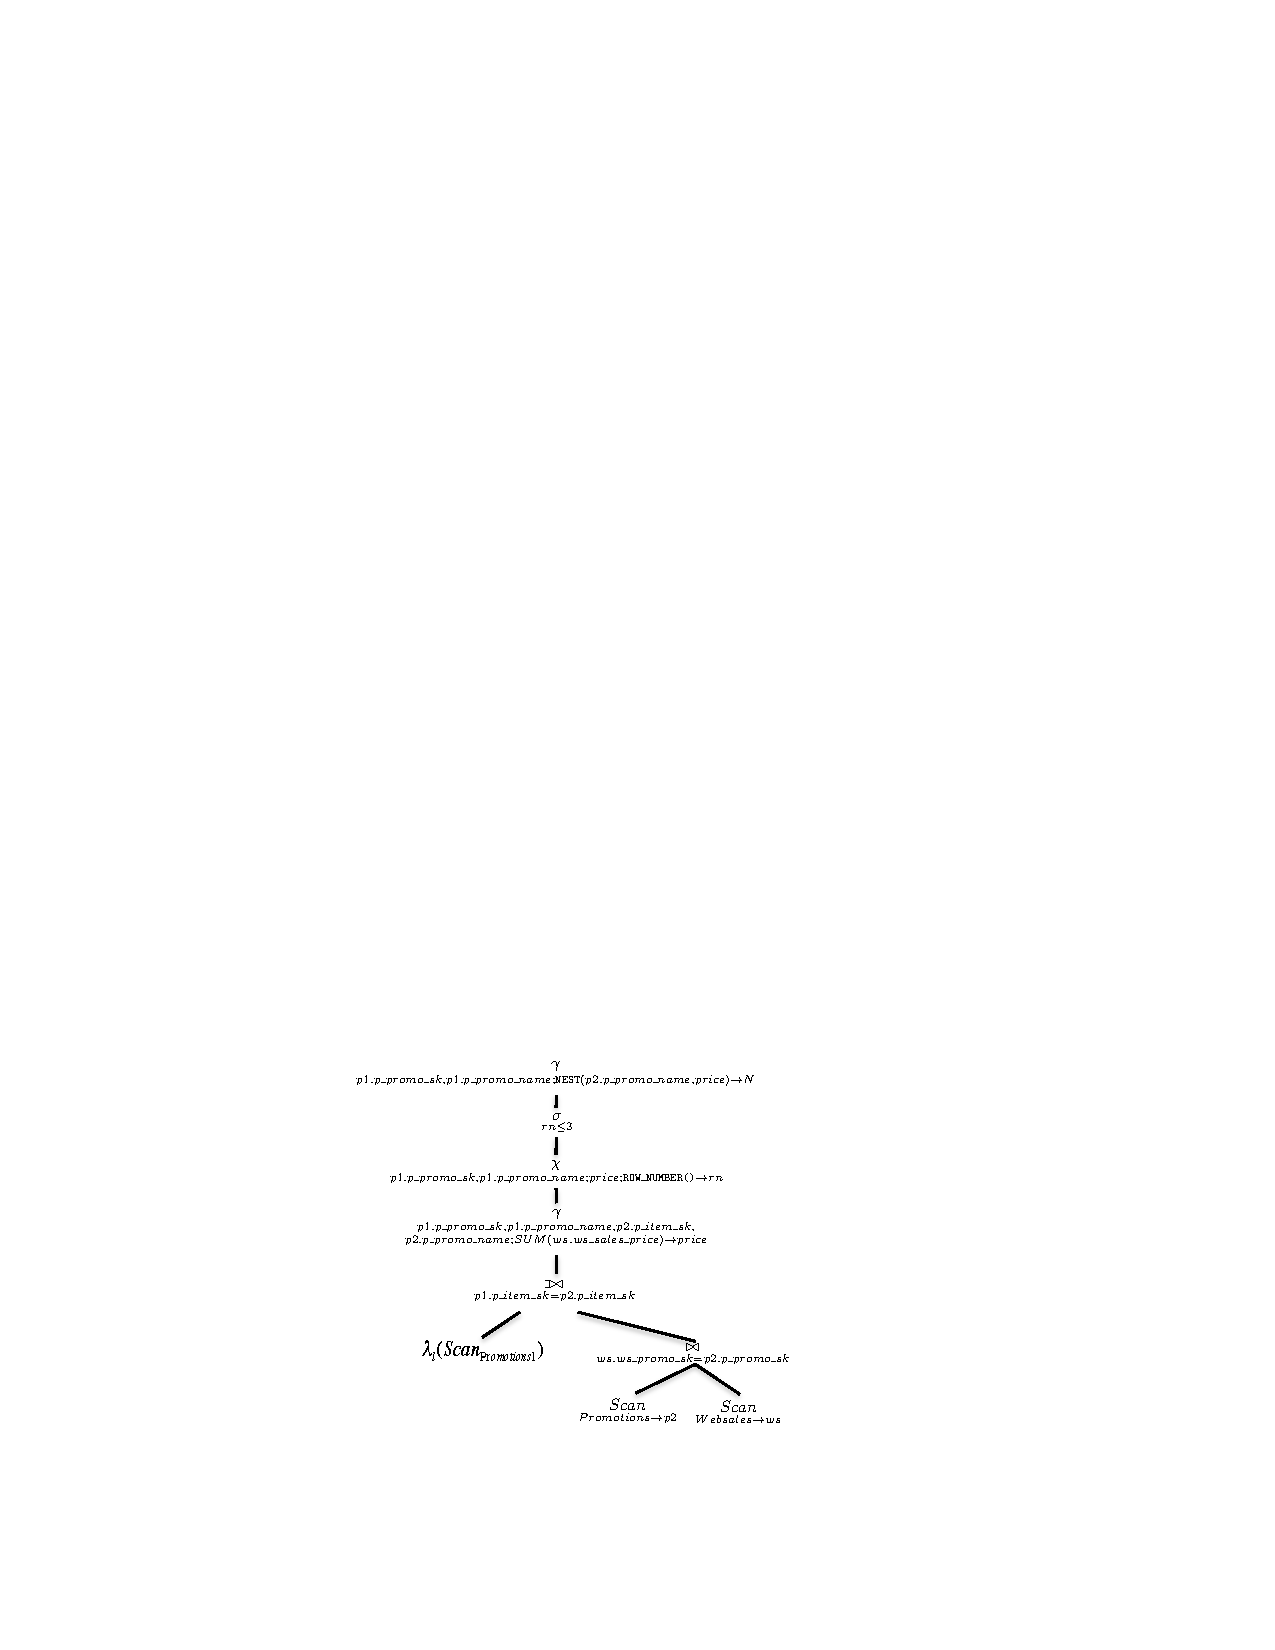
\includegraphics[width=1.05 \linewidth]{images/DSAAT_running-example.pdf}
\end{figure}

Notice that in the running example, there is a functional dependency from the correlated attribute \texttt{p\_item\_sk} to the attributes \texttt{p\_promo\_name} and \texttt{price} of \texttt{top\_web\_sales}. The $\leftouterjoin$ denormalizes intermediate results by joining on \texttt{p\_item\_sk}, thus introducing more non-correlated attributes from its left hand side. This creates two types of performance penalties: 1) horizontal redundancy: the $\leftouterjoin$ operator outputs unnecessarily wide tuples due to the additional $p1.p\_promo\_name$ attribute (which isn't used until the $\gamma_\texttt{NEST}$ operator), which increases the cost of the $\gamma_\texttt{SUM}$ and $\chi$ operators; 2) vertical redundancy: the $\leftouterjoin$ operator outputs redundant tuples if the correlated attribute $p1.p\_item\_sk$ is not unique, which also unnecessarily increases operator costs. Moreover, it introduces a requirement that the tuples from the output of left hand side of the left outer join be unique, since a key is required to process  the $\gamma$ and $\chi$ operators. In the running example, the key is $p1.p\_promo\_sk$.

\jules{Show NSAAT and how it improves upon DSAAT by outlying performance improvements.}

We introduce a normalized-set rewriting on figure \ref{NSAAT_example}. It introduces the $Scan$ and $\delta$ operators (which is reminiscent of the classical semi-join technique in distributed query processing), and deferring the $\leftouterjoin$ until all analytical operators are processed.

\begin{figure}[h]
\centering
\caption{Normalized Set-At-A-Time execution \label{fig:NSAAT_example}}
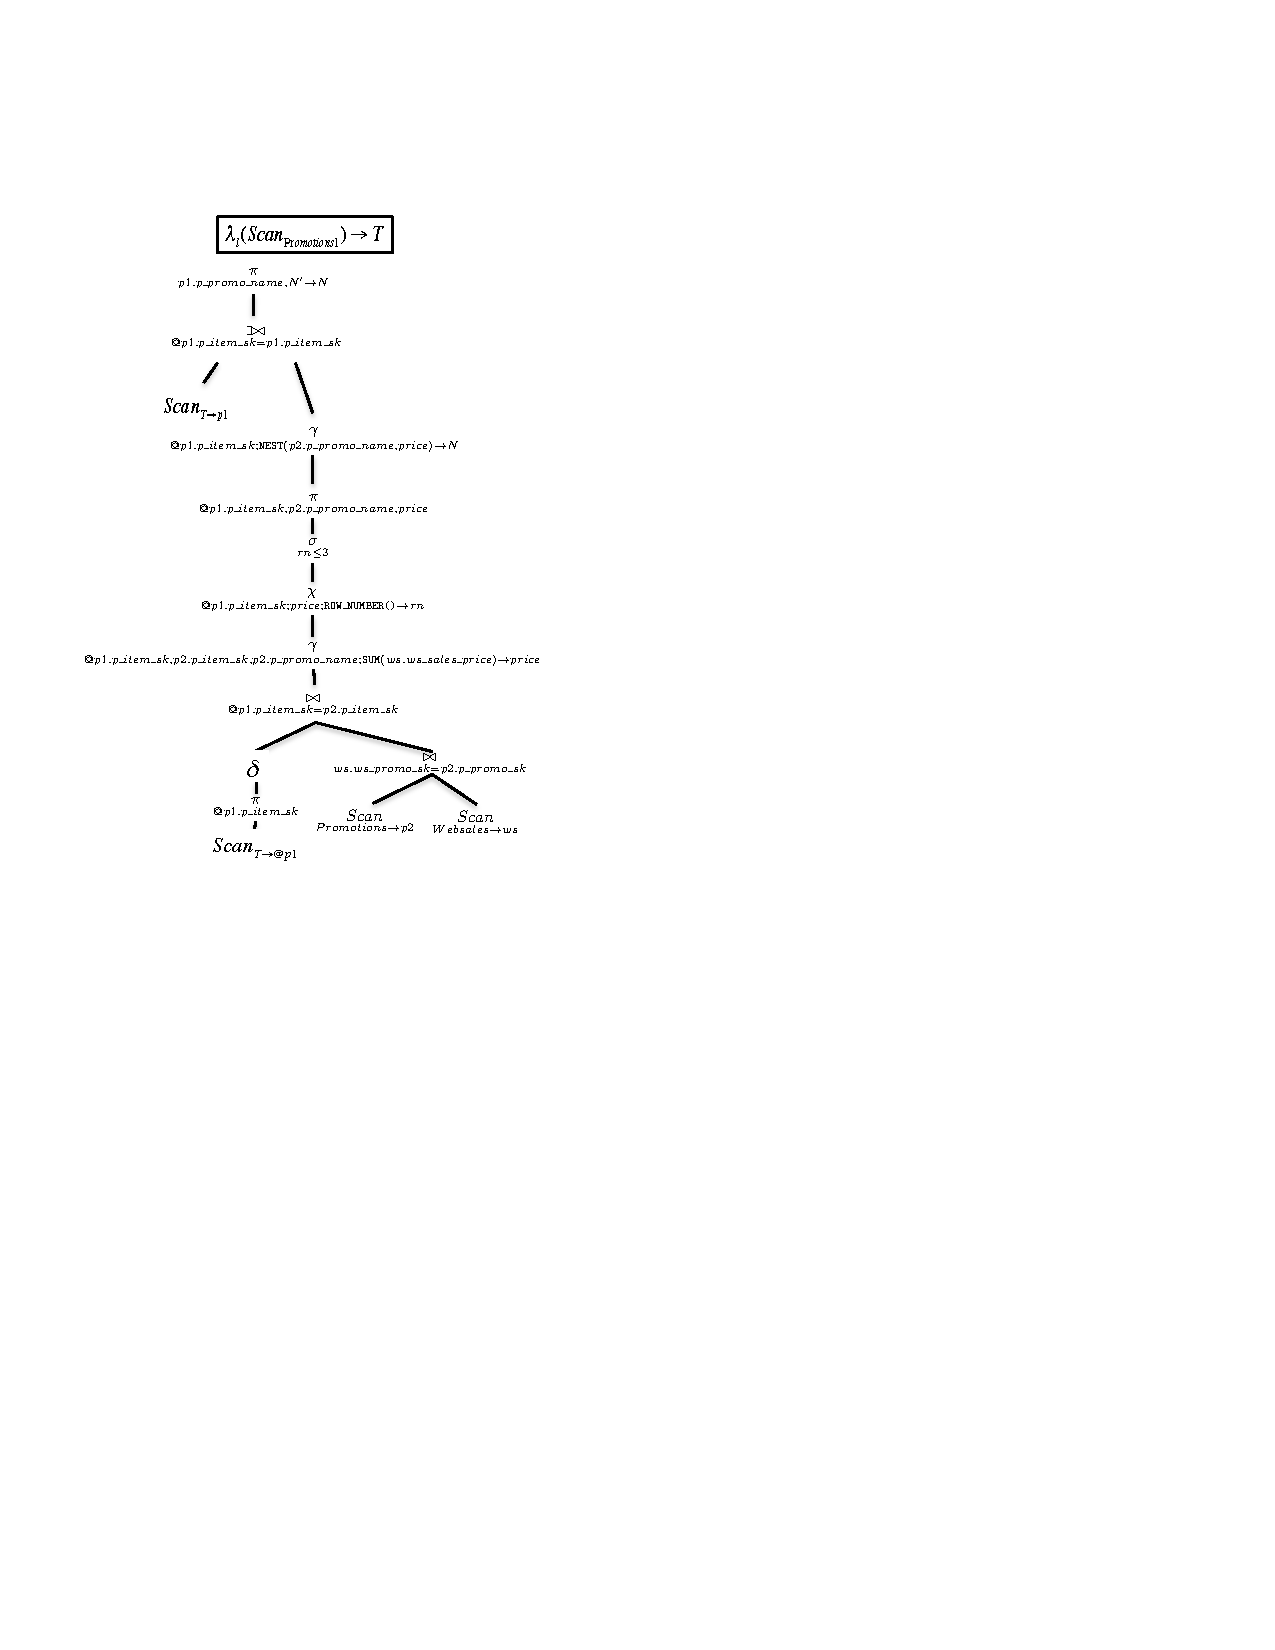
\includegraphics[width=1.05 \linewidth]{images/NSAAT_running-example.pdf}
\end{figure}

\jules{Outline and contributions}


\jules{The key requirement for DSAAT is only necessary because the $\gamma_{\texttt{NEXT}()}$ is happening above the left outer join. If the $\gamma_{\texttt{NEXT}()}$ is placed below the left outer join, the key requirement is no longer necessary but the performance may degrade because aggregation happens before the left outer join, which may be filtering}

\jules{@Yannis: One question that could arise is whether it is necessary that the input data to the query be relational, since it is in our running example. In particular, what happens if the correlation attributes are nested or missing for some or all tuples.}

\jules{The May paper \cite{may:2003aa}  uses the $\chi$ symbol for their apply plan operator and the $\alpha$ symbol to mean the head of a list. I hope our use of the same symbols for different operators won't confuse our readers early on.}

\jules{Unfortunately, there is no equivalent to the  \texttt{LIMIT} keyword in the SQL standard, each DBMS having it's own syntax. My introduction assumes the semantics of \texttt{LIMIT} are obvious.}

\section{Data Model and Algebra}

% SQL++ Data Model

In this paper, we use the SQL++ semi-structured data model and query language \cite{ong:2014aa}. We only retain here the most relevant features for our setting. The complete version of the language is available in \cite{ong:2014aa}.

\subsection{The SQL++ data model}

SQL++ queries input and output collections of values. Formally,  a {\em SQL++ value} is either
\begin{compact_enum}
	\item a {\em primitive value}, such as the string {\tt `abc'} or the integer {\tt 7}.
	\item a {\em tuple} $\{ a_1: v_1, \ldots, a_n: v_n \}$, where the attribute names $a_1,\ldots,a_n$ are strings and each attribute value $v_i$ is a SQL++ value.
	\item a {\em collection} $[ v_1, \ldots, v_n ]$, where each $v_i$ is recursively a SQL++ value. A collection may be ordered (then called an \emph{array}) or unordered (then called a \emph{bag}).
	\item the {\tt null} value.
%	\item the {\tt missing} value.
\end{compact_enum}

% SQL++ Query Language
\subsection{The SQL++ Query Language}

The SQL++ language is backwards compatible with SQL. As such, we define its semantics by \emph{removing} semantic restrictions from SQL:

\begin{itemize}
\item Unlike SQL's \texttt{FROM} clause variables, which bind to tuples
only, the \texttt{FROM} clause variables of SQL++ may bind to any
arbitrary SQL++ value.
\item  SQL++ is fully composable in the sense that subqueries
can appear anywhere, potentially creating nested results
when they appear in the \texttt{SELECT} clause.
\item Unlike SQL's aggregate functions which output scalar values, SQL++'s aggregate function may output any value. Of particular interest to the optimizations presented in this paper is the \texttt{NEST}($e$) function, whose output is a collection. Formally, just like any aggregate function, it is evaluated on each group created by \texttt{GROUP BY} clause. For each group, it returns a collection in which each element corresponds to the evaluation of expression $e$ for one tuple of the group.
\item Since SQL++ tuples may have attributes whose value is itself a tuple with attribute of its own, SQL++ allows path navigation of arbitrary depth. Formally, a \emph{tuple path navigation} $t.a$ from a tuple $t$ with existing attribute $a$ returns the value of $a$ in $t$. If $a$ does not exists in $t$, then $t.a$ returns the \texttt{null} value. \jules{I don't believe \texttt{MISSING} is required for this rewriting.}
\end{itemize}

\textbf{Tuple-at-a-time and Set-at-a-time nesting} Notice that a SQL++ query that produces nested collections can be formulated in two ways: either using a nested query in the \texttt{SELECT} clause, or using the \texttt{NEST()} aggregate function. In the first case, the nested query evaluating to a nested collection is evaluated for each tuple of the main query individually, and therefore we call this query formulation tuple-at-a-time nesting. In the second case, the nested collections are created all at once by the \texttt{GROUP BY} clause, and therefore we call this query formulation set-at-a-time nesting.

\subsection{The query pattern}

We consider here SQL++ queries which exhibit the following pattern :

% We could show how SQL++ running examples belong to the query pattern.
\lstinputlisting[language=SQL,label={list:query-pattern},caption={Query Pattern},escapeinside={(*}{*)}]{code/query_pattern.sql}

On listing \ref{list:query-pattern}, we denote lines 1, 15 and 16 to be the \emph{outer query}, and lines 2-14 to be the \emph{inner query}. The \texttt{SELECT} clause items other than the inner query and the SQL clauses below and including the outer query's \texttt{FROM} clause may contain any arbitrary SQL++ expression, thus are only shown as $\dots$ on the code fragment above. 
The inner query has the following characteristics:

% The query pattern should exhibit the characterization of the rewriting.
\begin{enumerate}
\item the variables produced by the outer query which may be in any SQL++ expression in the inner query. We will denote those variables as $c_1, \dots, c_n$. 
\item \jules{@Yannis: The original draft for this paper also included in the input pattern to the rewriting a list of zero of more assignments $CS_1 \leftarrow E_1, \dots, CS_p \leftarrow E_p$ in which $E_1, \dots, E_p$ are plans, possibly correlated with variables from the outer plan. I left them out here. We could add them through a \texttt{WITH} clause in the query pattern.}
\item The inner query may contain any of the following SQL++ clauses : \texttt{WHERE}, \texttt{GROUP BY}, \texttt{PARTITION BY}, \texttt{HAVING}, \texttt{ORDER BY}, \texttt{LIMIT}. Moreover, the items in any of those clauses may be any arbitrary SQL++ expression. \jules{@Yannis: the \texttt{OVER} and \texttt{PARTITION BY} clauses on figure \ref{list:query-pattern} are not mentioned in the SQL++ query language paper \cite{ong:2014aa}. I don't know if we can just put them there without further introduction.}
\item In the \texttt{SELECT} clause, expressions $a_1, \dots, a_m, w_1, \dots, w_l$ may be arbitrary SQL++ aggregation functions bound to variables $A_1, \dots, A_m, W_1, \dots, W_l$ respectively. Moreover, $P_1, \dots, P_k$ may be any nested queries bound to variables $N_1, \dots, N_k$ (These won't be rewritten away by the rule, and need subsequent calls to the rewriting rule to be removed from the plan.). Finally, $p_1, \dots, p_q$ may be arbitrary expressions bound to variables $u_1, \dots, u_q$.
\item The \texttt{FROM} clause expression $\hat{F}(c_1, \dots, c_n)$ may either be: (i) a single from item (name of a stored collection, collection literal, variable/path navigation mapped to a collection or a subquery) or (ii) any kind of join (\texttt{LEFT|RIGHT|FULL INNER|OUTER|CROSS JOIN}) (for conciseness we consider the cross product a special kind of join) between two items supported in the \texttt{FROM} clause, recursively. In both cases, if some from items are themselves subqueries or joins, these subqueries can be correlated through the attributes $c_1, \dots, c_n$. 
\end{enumerate}


% SQL++ Operators

\subsection{The SQL++ Algebra}

% SQL++ is a semi-structured query language which 
We present here an algebra for SQL++. This is a purely logical algebra, and physical execution of this algebra is discussed further in section 5. An algebraic plan $P = T_1 \leftarrow e_1 ; \ldots ; T_n \leftarrow e_n; e$ starts with a list of zero or more assignments $T_i \leftarrow e_i$, where each $T_i$ is a {\em temporary result} and each $e_i$ is a SQL++ algebra expression that may use the previously computed temporaries $T_1, \ldots, T_{i-1}$. The result of $P$ is the SQL++ collection resulting from the evaluation of the {\em result expression} $e$, which may use any temporary $T_1, \ldots, T_n$.

% Maybe discuss logical plan here
The algebraic operators involved in the SQL++ algebra expressions input and output a collection (called binding collection) of tuples (called binding tuples). This collection may be ordered (then called an array) or unordered (then called a bag). Each binding tuple maps accessible variables (i.e. variables in the scope) to their corresponding value. Each value may itself by any SQL++ value (including a tuple or a collection).

The majority of SQL++ algebra operators are extensions of operators well-known from conventional SQL processing (cf. textbooks \cite{Garcia-Molina:2008:DSC:1450931}). While conventional operators input and output collection of tuples with primitive or scalar attribute values, SQL++ extends algebraic operators to allow the binding attribute values to also be tuples and collections.

The list of standard operators comprises CartesianProduct (or CrossProduct) $\crossproduct$, Union $\cup$, Intersection $\cap$, Difference $-$, Selection $\select_c$, InnerJoin $\innerjoin_c$, FullOuterJoin $\fullouterjoin_c$, LeftOuterJoin $\leftouterjoin_c$, SemiJoin $\semijoin_c$, AntiSemiJoin $\antisemijoin_c$, Projection $\project_{p_1 \rightarrow u_1, \dots, p_q \rightarrow u_q}$, Sort $\sort_{o_1, \dots, o_j}$ (where $o_1, \dots, o_j$ is the list of ordering terms, which initially appears in the SQL++ \texttt{ORDER BY} clause), limit $\lambda_l$ (which outputs the first $l$ binding tuples of its input), duplicate elimination $\distinct$, group-by $\groupby_{g_1, \dots, g_i; a_1(.) \rightarrow A_1, \ldots, a_m(.) \rightarrow A_m}$ (where $g_1, \dots, g_i$ is the list of grouping terms, which initially appears in the \texttt{GROUP BY} clause and $a_1, \ldots, a_m$ are the aggregate functions, which initially appear in the \texttt{HAVING} and \texttt{SELECT} clauses).

In the remainder, given a binding tuple $t$, an attribute name $a$ that is not already the name of a binding attribute of $t$ and a value $v$, the notation $t\#{a : v}$ denotes the tuple that has all the attribute name/value pairs of $t$ as well as the attribute name $a$ mapped to the value $v$.

The \textbf{Ground} operator $\ground$ is the only accepted leaf of a plan. It always outputs a single empty binding tuple $\{ \}$. 

The \textbf{Scan} operator $\scanop_{S \mapsto s}$ is used to iterate over collections. For each input binding tuple $t$, it iterates over the collection $C$ bound to $S$ and for each element $v \in S$, it outputs the binding tuple $t \# \{ s:v \}$. Notice that if the child of Scan is a Ground, it really behaves like an iterator over the collection $S$ (in such cases we do not write Ground explicitly, for conciseness). However, if it is any other operator (e.g. another Scan), it unnests the collection $C$ with respect to each input binding tuple.

The \textbf{ApplyPlan} operator $\applyplan_{P \mapsto N}$ is the algebraic counterpart of tuple-at-a-time nesting. For each input binding tuple $t$, the ApplyPlan operator evaluates the plan $P$ to a value $v$ and outputs the tuple $t \# \{ N: v \}$. In general, $P$ is a correlated plan $P(t)$, such that variables of the input binding tuples appear as \textit{parameters} in $P$ wherever constants or variables can appear in uncorrelated plans. In this case, each $v$ is the result of evaluating $P\backslash t$, i.e. the plan $P$ in which all the parameters have been replaced by their corresponding value for the current binding tuple $t$. Notice that if $P$ corresponds to a standard \texttt{SELECT} query, each $v$ is a collection and the ApplyPlan effectively nests a collection in every binding. If a SQL++ clause $C$ requires the evaluation of a nested query $SQ$ (e.g. $\texttt{SELECT (}SQ\texttt{) AS s ...}$), the algebraic translation $\operatorname{alg}(C)$ of this clause is composed of the corresponding SQL++ operator on top of an ApplyPlan (e.g. $\project_{\_v \mapsto s}(\applyplan_{\operatorname{alg}(SQ) \mapsto \_v}(\ldots))$). Notice that this corresponds to an eager evaluation of nested queries, since all the nested queries used by an operator are evaluated before the operator itself. This algebraic translation does not produce correct results when the nested queries are used by short-circuiting functions (e.g. \texttt{CASE WHEN}, \texttt{AND}) and possibly produce runtime errors (e.g. division by zero), but in our experience such use cases are very uncommon. The treatment of such nested queries are out of the scope of this paper.

% SQL++ TAAT plan
The \textbf{GroupBy} operator $\groupby_{g_1,\ldots,g_i; a_1(.) \mapsto A_1, \ldots, a_m(.) \mapsto A_m}$ behaves like SQL's grouping operator: it partitions the input binding tuples according to the evaluation $v_{g_1},\ldots, v_{g_i}$ of the grouping expressions $g_1,\ldots,g_i$, computes the evaluation $v_{A_1},\ldots,v_{A_m}$ of the aggregate functions $a_1,\ldots,a_m$ on each partition and outputs, for each partition, the binding tuple $\{g_1: v_{g_1}, \ldots, g_i: v_{g_i}, A_1: v_{A_1}, \ldots, A_m: v_{A_m}\}$. SQL++ extends SQL by allowing aggregate function that return complex values, such as the \texttt{NEST(}$e$\texttt{)} aggregate function. This particular function returns, for a given partition of input binding tuples, a collection of tuples which includes the evaluation $e(t)$ for each input binding tuple $t$ in that partition. Using \texttt{NEST()} as aggregate function in the GroupBy operator is the algebraic counterpart of set-at-a-time nesting. 

Like in SQL, total aggregation queries, that is, queries with aggregations in the \texttt{SELECT} clause but no \texttt{GROUP BY} clause (e.g. \texttt{SELECT count(*) FROM customers}) correspond to a special version $\groupby^T_{a_1(.) \mapsto A_1, \ldots, a_m(.) \mapsto A_m}$ of the GroupBy operator. $\groupby^T_{a_1(.) \mapsto A_1, \ldots, a_m(.) \mapsto A_m}$ behaves like $\groupby_{a_1(.) \mapsto A_1, \ldots, a_m(.) \mapsto A_m}$ (a GroupBy operator without grouping attributes, that creates a single partition), with the following exception: if $\groupby$ inputs an empty binding bag, it outputs a empty binding bag, whereas if $\groupby^T$ inputs an empty binding bag, it outputs a binding bag with a single binding tuple containing default values $\operatorname{default}(f_i)$ for each aggregate function $f_1, \ldots, f_n$. For instance, $\operatorname{default}(\texttt{SUM()})$ is \texttt{null} and $\operatorname{default}(\texttt{COUNT()})$ is \texttt{0}.

The \textbf{PartitionBy} operator $\partitionby_{x_1,\dots,x_{n1}; oc; w(.) \mapsto W}$ enables support of the SQL 2003  \texttt{PARTITION} feature and window functions. In addition, $\partitionby$ is important for the optimizations discussed in this paper, as one of them introduces a $\partitionby$ operator in the rewritten plan (cf. Section~\ref{sec:NSAAT}). Formally, $\partitionby$ (i) partitions the input binding tuples according to the evaluation $v_{x_1},\ldots,v_{x_{n1}}$ of the grouping expressions $x_1,\ldots,x_{n1}$ then (ii) sorts the binding tuples within each partition according to the optional \texttt{ORDER BY} clause $oc$ (identical to a standard SQL \texttt{ORDER BY} clause, but only sorts the bindings within each partition) then (iii) computes the evaluation $v_W$ of the window function $w$ for each binding tuple of each partition and finally (iv) outputs, for each binding tuple $t$ of each partition, the binding tuple $t\#\{W: v_W\}$. For example:

\noindent \begin{tabular}{@{}c@{~~}c@{}}
    $\chi_{\texttt{nation}; \tau_{\texttt{sales}, \texttt{DESC}} ; row\_number() \mapsto \texttt{rank}}$\\
		$
    \left(~
    \begin{scriptsize}
    \begin{array}{|@{~}c@{~}|@{~}c@{~}|@{~}c@{~}|}
    \hline
    \textbf{nation} & \textbf{name} & \textbf{sales} \\ \hline
    \texttt{USA} & \texttt{Joe} & 6 \\ \hline
    \texttt{China} & \texttt{Fu} & 4 \\ \hline
    \texttt{China} & \texttt{Zhao} & 8 \\ \hline 
    \end{array}
    \end{scriptsize}
    ~\right)
    =$
&
    $\begin{scriptsize}
    \begin{array}{|@{~}c@{~}|@{~}c@{~}|@{~}c@{~}|@{~}c@{~}|}
    \hline
    \textbf{nation} & \textbf{name} & \textbf{sales} & \textbf{rank} \\ \hline
    \texttt{USA} & \texttt{Joe} & 6 & 1 \\ \hline
    \texttt{China} & \texttt{Zhao} & 8 & 1\\ \hline
    \texttt{China} & \texttt{Fu} & 4 & 2\\ \hline
    \end{array}
    \end{scriptsize}
    $
\\
\end{tabular}\\

\section{Algebraic Formulations}

\subsection{Tuple At A Time}

On figure \ref{fig:R0} is shown an algebraic plan corresponding to a direct translation of the query pattern into SQL++ algebra, which we denote as the \emph{tuple-at-a-time} (TAAT) algebraic formulation. This plan is the plan which semi-structured databases would generate initially, before any algebraic rewriting optimizations are performed. For this reason, we also call this formulation the initial plan. The plan on the left side of the figure corresponds to the translation of the outer query (denoted \emph{outer plan}), while the plan (denoted as $P$) in the dashed-lined box is the translation of the inner query (denoted as \emph{inner plan}). 

% \jules{Ensure that path variables are not used in algebra}

% Describe the outer query expression
\textbf{Outer Plan} The expression $E$ of the outer plan corresponds to the algebraic translation of the outer query SQL clauses below and including the \texttt{FROM} clauses, while the expression $G$ is the translation of the \texttt{SELECT} clause items other than the inner query. The apply plan operator $\alpha$ is correlated by variables $c_1, \dots, c_n$ while $z_1, \dots, z_{q'}$ are those variables produced by $E$ which are required by operators in $G$.

% Describe the inner query expression
\eat{
\textbf{Inner Plan} Within the inner plan (denoted as $P(c_1, \dots, c_n$), the translation of the \texttt{FROM} clause is shown on table \ref{table:taat-from}. It is defined recursively, where the value of $F(c_1, \dots, c_n)$ is translated into either: 1) a stored collection $R$, 2) a \texttt{FROM} item expression corresponding to the translation of a subquery (which recursively can have the $P$ normal form)correlated by attributes in $C_{subquery}$, itself a subset of $\{c_1, \dots, c_n\}$ 3) any kind of join ($\crossproduct$, $\innerjoin$, $\fullouterjoin$, $\leftouterjoin$, $\rightouterjoin$, etc.) between two \texttt{FROM} item expressions $F_{left}$, $F_{right}$ correlated by attributes in $C_{left}$, $C_{right}$, respectively. Note that any of $C_{subquery}, C_{left}, C_{right}$ could be empty, in which case the \texttt{FROM} item would be uncorrelated.
\begin{table}[]
\centering
\caption{Value of $F(c_1, \dots, c_n)$ \label{table:taat-from}}
\begin{tabular}{C{3cm} C{4cm}}
1) Stored collection   & $Scan_{R \mapsto r}$  \\
2) Subquery  & $F_{subquery}(C_{subquery})$  \\
3) Join between two \texttt{FROM} item & $Join_c(F_{left}(C_{left}),F_{right}(C_{right})$ \\
\end{tabular}
\end{table}
}

\textbf{Inner Plan} Within the inner plan (denoted as $P$), the value of $F(c_1, \dots, c_n)$ corresponds to the translation of the \texttt{FROM} clause expression $\hat{F}(c_1, \dots, c_n)$.  Next, operators $\sigma_w$, $\groupby_{g_1,\ldots,g_i; a_1(.) \mapsto A_1, \ldots, a_m(.) \mapsto A_m}$, $\sigma_h$, $\tau_{o_1, \dots, o_j}$, $\lambda_l$ correspond to the algebraic translation of the query pattern's \texttt{WHERE}, \texttt{GROUP BY}, \texttt{HAVING}, \texttt{ORDER BY} and \texttt{LIMIT} clauses, respectively. Finally, operators $\partitionby_{x_1^1,\dots,x_{n1}^1; oc^1; w^1(.) \mapsto W^1}$, $\dots$, $\partitionby_{x_1^l,\dots,x_{nl}^l; oc^l; w^l(.) \mapsto W^l}$, $\alpha_{P_1 \mapsto N_1}, \dots, \alpha_{P_k \mapsto N_k}$ correspond to the \texttt{PARTITION BY} statements and subqueries present in the \texttt{SELECT} clause.

\jules{@Yannis: one tricky thing to notice here is the position of the Apply plan ($\alpha$) operators, which reflect here the possible presence of nested queries in the input's \texttt{SELECT} clause. However, given we allow any arbitrary SQL++ expression in the \texttt{WHERE}, \texttt{GROUP BY}, etc clauses, we could, for example, have a subquery in the \texttt{WHERE} clause. Those would not be accounted for in this translation of the plan.}

\begin{figure}[h]
\centering
\caption{Tuple-At-A-Time Formulation (TAAT) \label{fig:R0}}
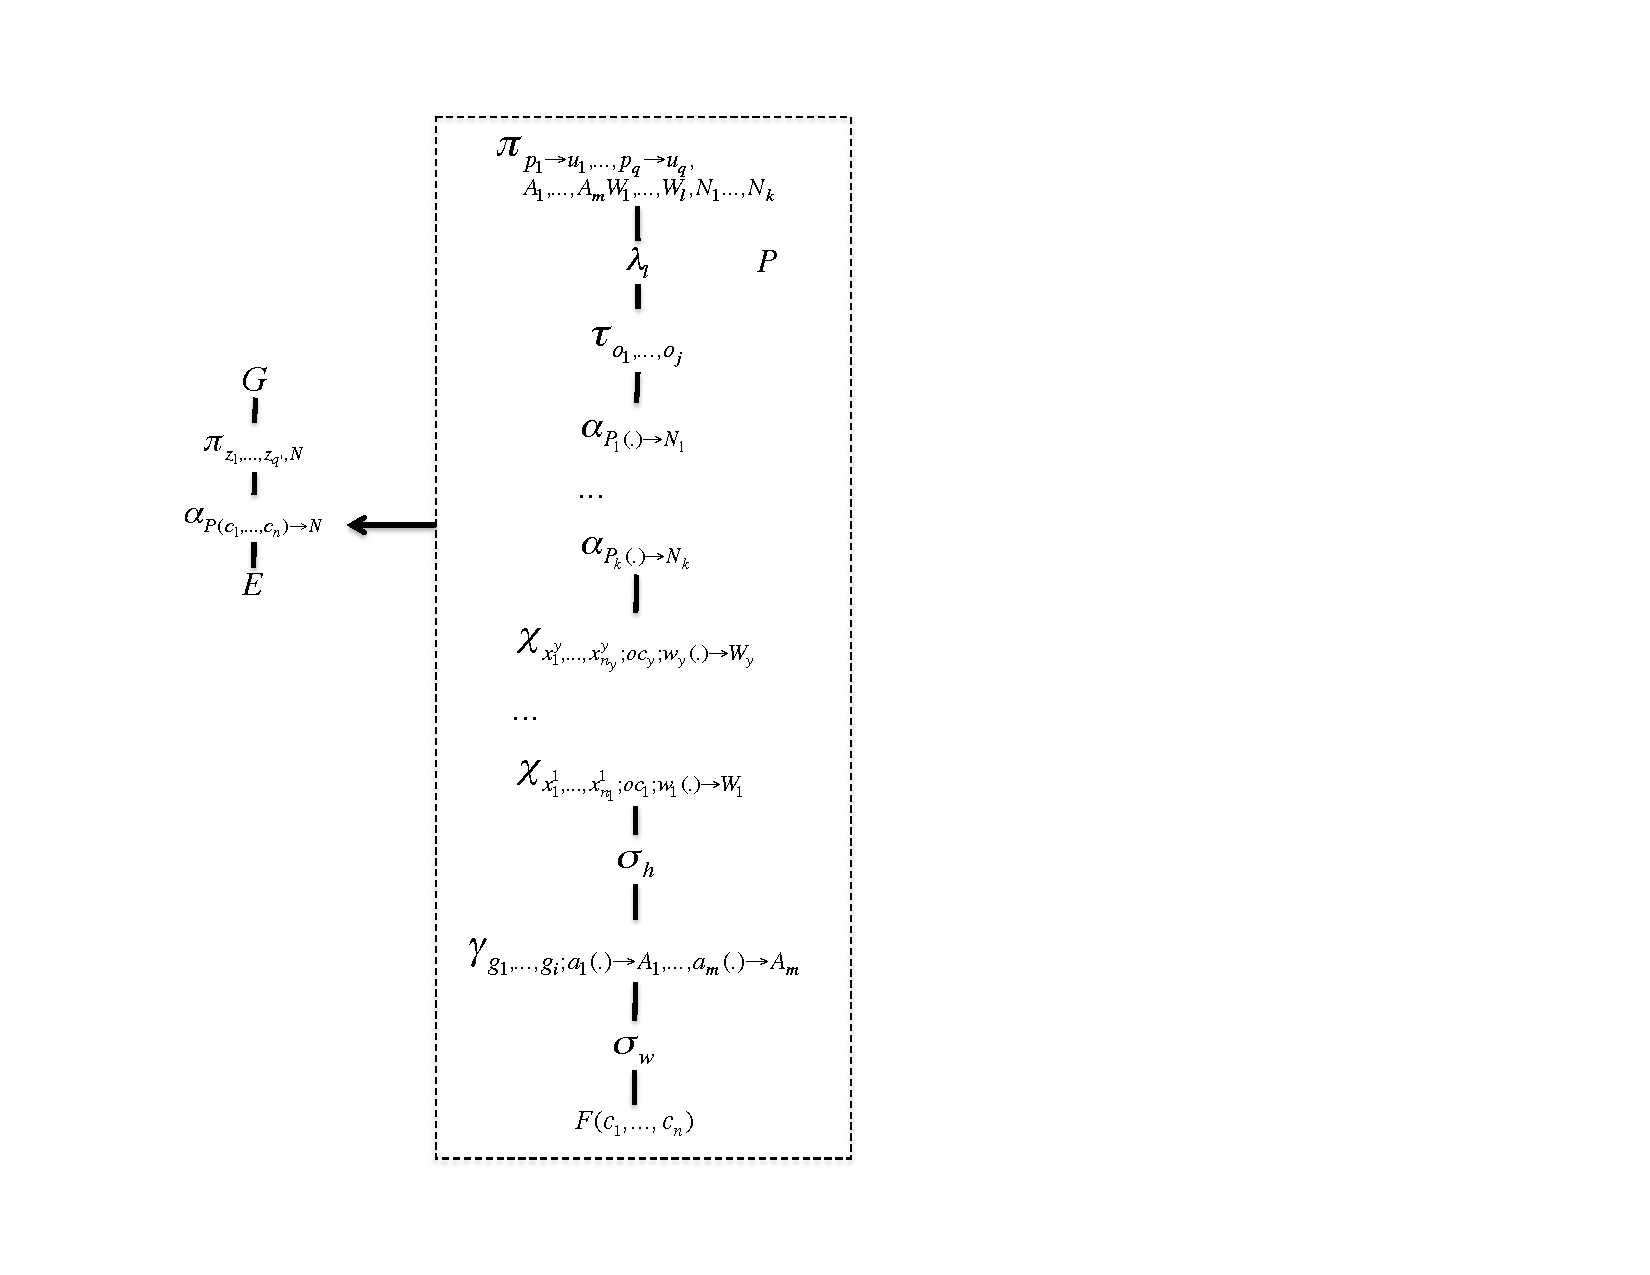
\includegraphics[width=0.85 \linewidth]{images/R0.pdf}
\end{figure}

The tuple-at-a-time formulation shown above constitutes only one way to formulate the query pattern. In particular, it evaluates the inner plan $P$ once for every binding tuple in the output of $E$. We present next two alternative algebraic formulations which evaluate the inner query for every binding tuple at the same time, which we denote as a set-at-a-time execution. We distinguish the \emph{normalized} and \emph{denormalized} set-at-a-time executions.

\subsection{Normalized Set-at-a-time \label{sec:NSAAT}}

The normalized set-at-a-time (NSAAT) formulation of the query pattern is shown on the figures \ref{fig:R2} and \ref{fig:from-items}. We obtain this formulation by rewriting the tuple-at-a-time formulation. Instead of evaluating a very similar (only differing by the value of the correlated attributes) inner query for each tuple in the output of $E$, it will (i) introduce a cross product between $E$ and the leaves of the inner plan $P(c_1, \dots, c_n)$ (ii) execute the inner plan only once on the output of this cross product (iii) group the tuples in the output of this inner plan according to the tuple of $E$ they correspond to (iv) create the nested collections using the \texttt{NEST()} aggregate function (v) join back with the original $E$ to preserve cardinality. Thus, the normalized set-at-a-time formulation replaces the tuple-at-a-time nesting operator $\alpha$ with a set-at-a-time nesting operator $\gamma_{\texttt{NEST}}$. The details of the rewriting are as follows:

\begin{figure}[h]
\centering
\caption{Normalized Set-At-At-Time Formulation (NSAAT) \label{fig:R2}}
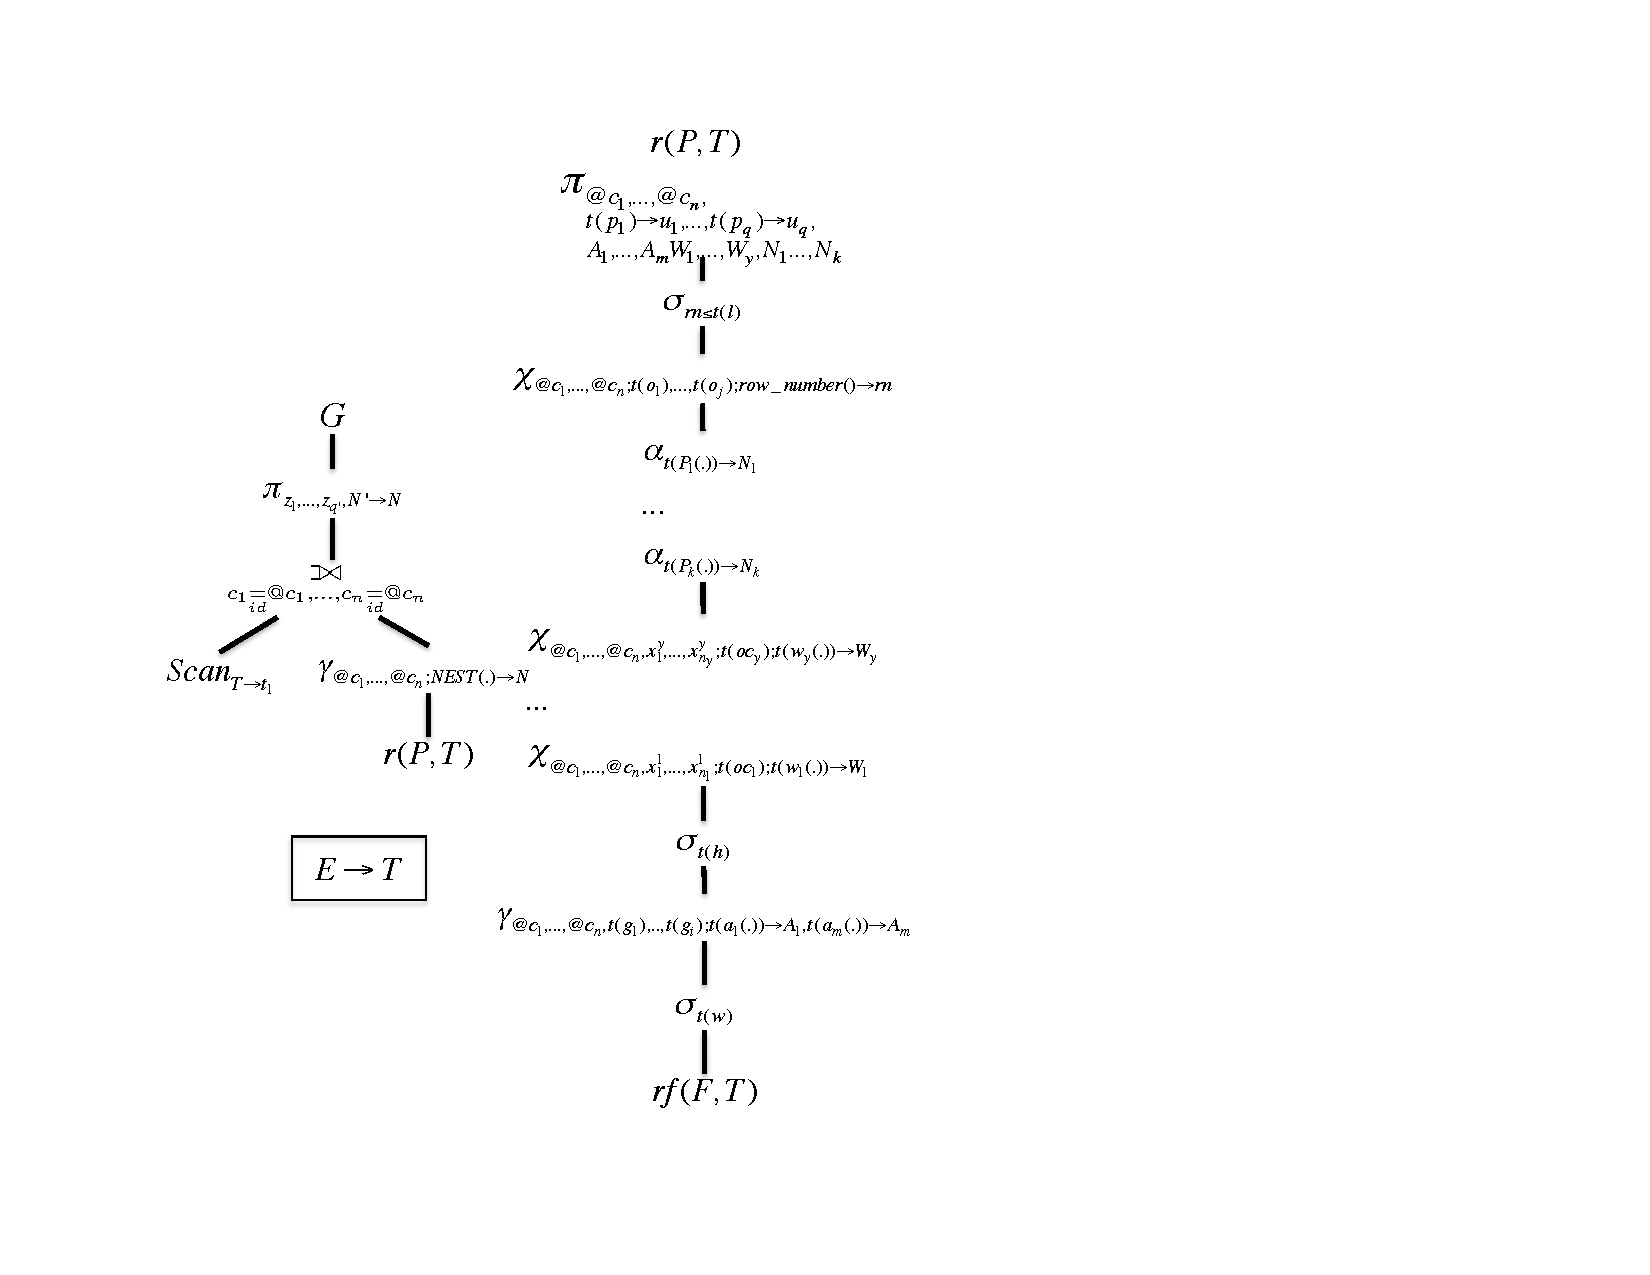
\includegraphics[width=\linewidth]{images/R2.pdf}
\end{figure}

% Outer Plan
\textbf{Outer Plan} The rewriting of the outer plan is shown on figure \ref{fig:R2}. The output of $E$ is assigned to a temporary table $T$. The plan $P$ is rewritten to $r(P,T)$ (as explained below). The result of this rewritten plan goes to a $\gamma_{\texttt{NEST(.)}}$ operator that groups according to the correlated attributes $c_1, \dots, c_n$ and nests all the binding tuples with the same correlated values. As we will see next, the group of binding tuples nested with a given set of correlated values $v_{c_1}, \dots, v_{c_n}$ corresponds exactly to those bindings which would be outputted by the original $P$ if parameterized with values  $v_{c_1}, \dots, v_{c_n}$. Next, a $\leftouterjoin$ operator joins this back with the original $T$ and a final $\pi$ operator ensures that the extra attributes created by the outer join are projected out. $\pi$ also replaces the \texttt{null} values introduced by the outer join with empty collections (in the figure, $N'$ stands for the translation of the SQL++ statement \texttt{CASE WHEN N IS NULL THEN [] ELSE N}). Note that if the original inner plan is a total aggregation query, the $\gamma^T_{a_1(.) \rightarrow A_1, \dots, a_m(.) \rightarrow A_m}$ is rewritten into $\gamma^T_{c_1, \dots, c_n; a_1(.) \rightarrow A_1, \dots, a_m(.) \rightarrow A_m}$. In this case, the top $\pi$ operator replaces \texttt{null} $N$ bindings with a collection containing a single tuple with default values for each total aggregate function in the original query. \jules{The approach above could be problematic because it does not distinguish between the \texttt{null}s created by the outer join from the \texttt{null}s pre-existing on the right hand side. This is not a problem here because all binding tuples from the right hand side will have a non-null \texttt{N}}.

\begin{figure}[h]
\centering
\caption{\texttt{FROM} clause rewriting \label{fig:from-items}}
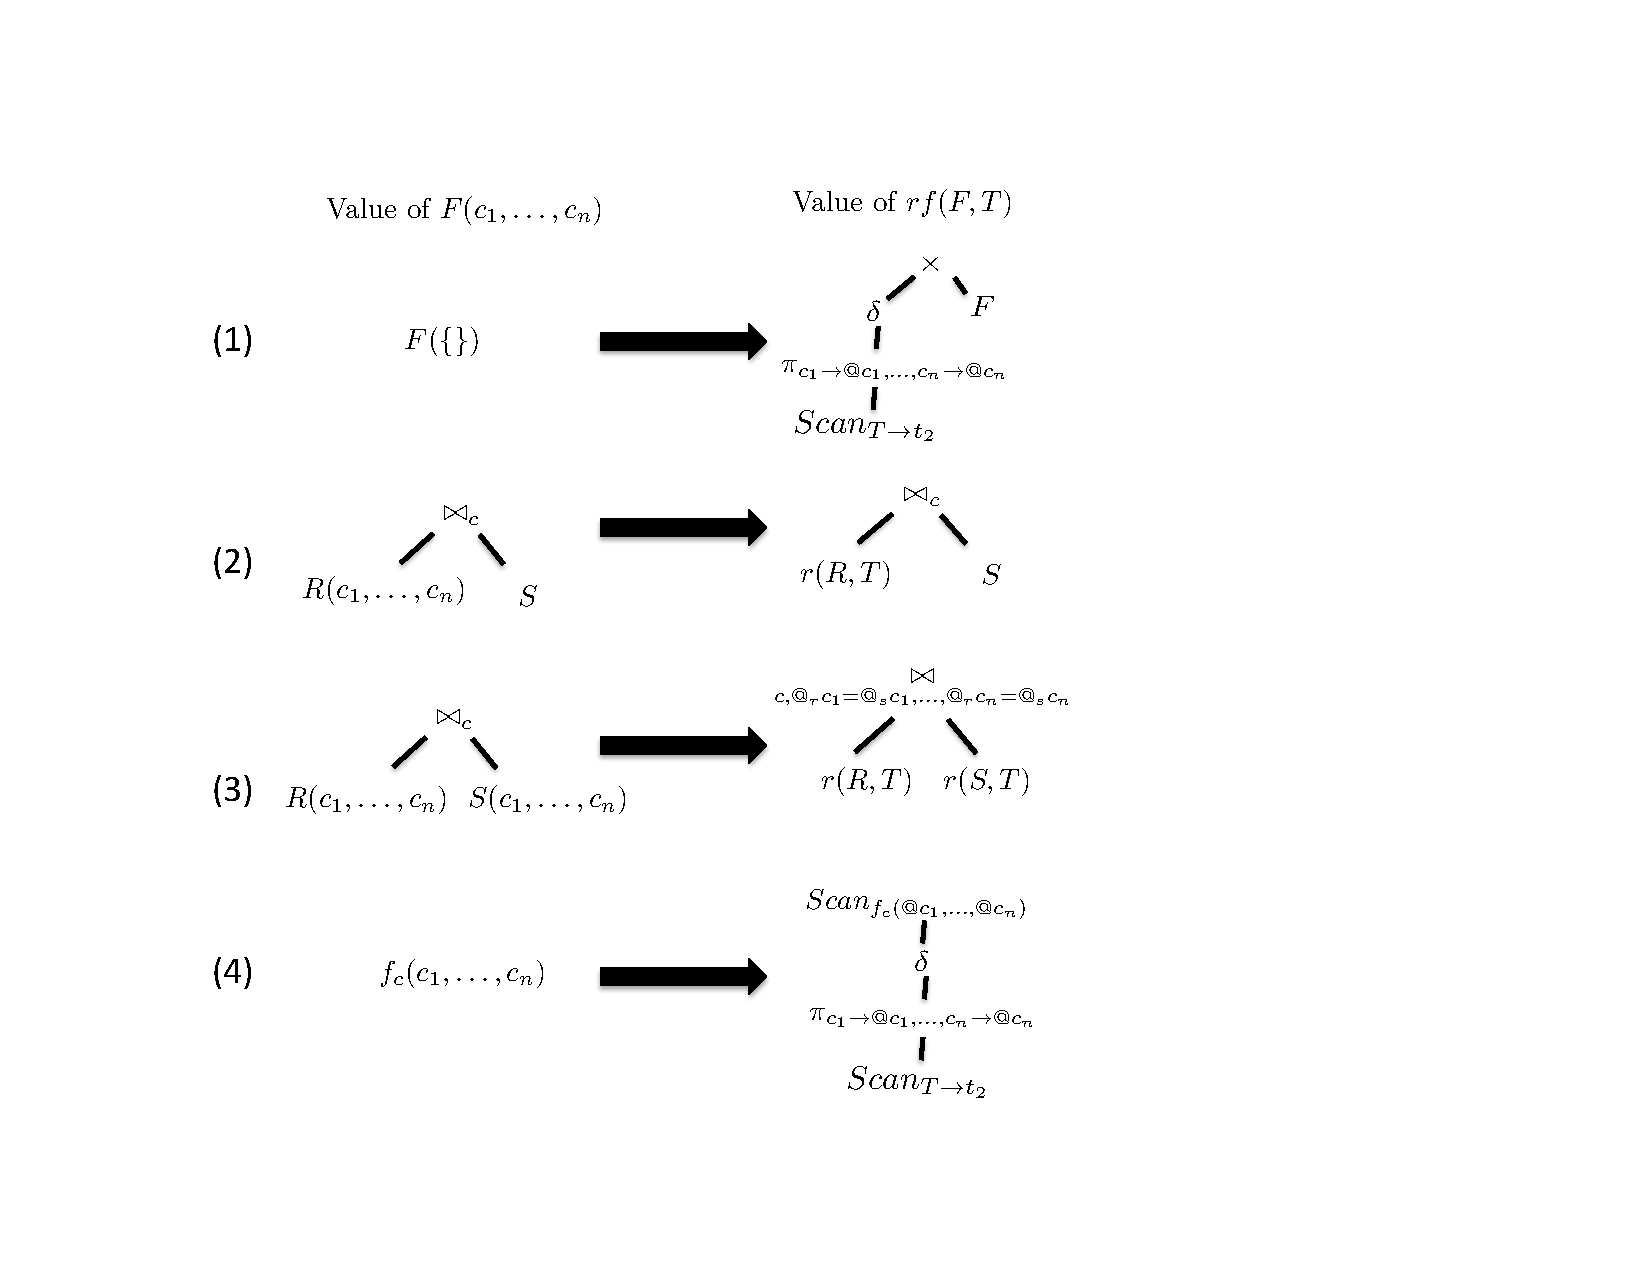
\includegraphics[width=\linewidth]{images/F_RF.pdf}
\end{figure}

We next describe how to rewrite the inner plan's \texttt{FROM} clause (figure \ref{fig:from-items}). The rewriting $r(P,T)$ of the nested plan $P$ introduces a cross product between the distinct correlated attributes of $T$ an the leaves of $P$. This is done by rewriting $rf(F,T)$ of the \texttt{FROM} clause $F$ of $P$. The rewriting of $F$ requires a case analysis (for conciseness, we treat $A \times B$ in the initial plan as $A \innerjoin_{true} B$ and do not explain it further): i) If $F$ is not correlated, it is rewritten into a simple cross product between $F$ and $\delta(\pi_{c_1, \dots, c_n}(T))$. A $\pi$ operator keeps only the correlated attributes $c_1, \dots, c_n$ renamed into $@c_1, \dots, @c_n$ (case 1 of figure \ref{fig:from-items}). ii) If $F$ is one correlated subquery $R(c_1, \dots, c_n)$, it is recursively rewritten into $r(R,T)$ (not shown in figure). iii) if $F$ is a join between two \texttt{FROM} items, but only one is correlated $R(c_1, \dots, c_n)$, then only $R$ is recursively rewritten into $r(R,T)$ (if it is a subquery) or $rf(R,T)$ (if it is a join).  iv) If $F$ is a join between two correlated branches $R(c_1,\dots,c_n)$ and $S(c_1,\dots,c_n)$, both are recursively rewritten to  $r(R,T)$ / $rf(R,T)$ and $r(S,T)$ / $rf(S,T)$ if they are subqueries/joins respectively. Moreover, the join condition $c$ is modified to enforce that the bindings outputted by the join correspond to the same values of correlated attributes on both sides (case 3 of figure \ref{fig:from-items}, $@$ symbols have additional subscripts to distinguish the renamings on the left and right hand side ).  v) If $F$ is a correlated expression (e.g. a path starting from a correlated variable and evaluating to a collection), it is rewritten into an unnesting Scan of $t(f_c(c_1, \dots, c_n))$ on top of $\delta(\pi_{c_1, \dots, c_n}(T))$. vi) Finally, if a join condition in $F$ is correlated, the rewriting corresponds to the case when both branches are correlated and the join condition is rewritten into $t(c)$ (not shown in the figure). Notice that the value of $rf(F,T)$ in cases (1) and (4) from figure \ref{fig:from-items}. The duplicate elimination is only required if there may be duplicate correlate attributes in the input.  In the case where the set of correlated attributes includes a key to the output of expression $E$ ($key(E) \subseteq \{c_1, \dots, c_n\}$), the $\delta$ operator can be eliminated.

% Inner Query
\textbf{Inner Plan} The rewriting of the inner plan $P$ is shown on figure \ref{fig:r2}. If $X$ is or an expression of plan $P$ correlated by attributes $c_1, \dots, c_n$, we denote $t(X)$ the same expression $X$ in which the attributes $c_1, \dots, c_n$ are substituted with variables $@c_1, \dots, @c_n$. i) The top $\pi$ operator of $P$ is modified to also output the attributes $@c_1, \dots, @c_n$ necessary for the $\gamma_{\texttt{NEST}(.)}$ and $\leftouterjoin$ operators above. iii) The nested plans $P_1, \dots, P_k$ of eventual $\alpha$ operators in $P$ are rewritten to $t(P_1), \dots, t(P_k)$. iv) The eventual $\tau$ and $\lambda$ operators are replaced with two other operators: on the one hand, a $\chi$ operator that groups according to $c_1, \dots, c_n$, orders according to the $t(o_1), \dots, t(o_j)$, then computes the row number of each tuple in its partition. The row number can then be used with a $\sigma$ operator to simulate the $\lambda$ (note that, depending on the implementation, if the $\gamma$ operator at the top of the rewritten plan breaks the ordering between the binding tuples coming from the $\chi$, the \texttt{NEST} function will have to sort again the tuples in each nested collection according to the row number). v) The grouping attributes of the eventual $\chi$ operators of $P$ are modified to also group by $@c_1, \dots, @c_n$. vi) The \texttt{HAVING} clause condition $h$ is rewritten to $t(h)$. vii) The grouping attributes of the eventual $\gamma$ operator of $P$ are modified to also group by $@c_1, \dots, @c_n$. viii) The \texttt{WHERE} condition $w$ is rewritten to $t(w)$.

\eat{
\begin{table}[]
\centering
\caption{Value of $rf(F,T)$ \label{table:saat-from}}
\begin{tabular}{C{3cm} C{3.5cm}}
1) Stored collection   & $\times(\delta(\pi_{c_1, \dots, c_n}(Scan{T \mapsto t_2})), Scan_{R \mapsto r})$  \\
2) Subquery  & $F_{subquery}(C_{subquery})$  \\
3) Join between two \texttt{FROM} item & $Join_c(F_{left}(C_{left}),F_{right}(C_{right})$ \\
\end{tabular}
\end{table}
}

\subsection{Denormalized Set-at-a-time}

The denormalized-set-at-a-time (DSAAT) formulation of the query pattern is shown on figure \ref{fig:R4}. We also describe this pattern rewriting of the TAAT formulation. 

% Where clause 

% Investigating further restrictions on the denormalized set-at-a-time.



% Restriction
$E$ has to be a set. It can't just be a 

\begin{figure}[h]
\label{fig:R4}
\centering
\caption{Denormalized Set-At-At-Time Formulation (DSAAT)}
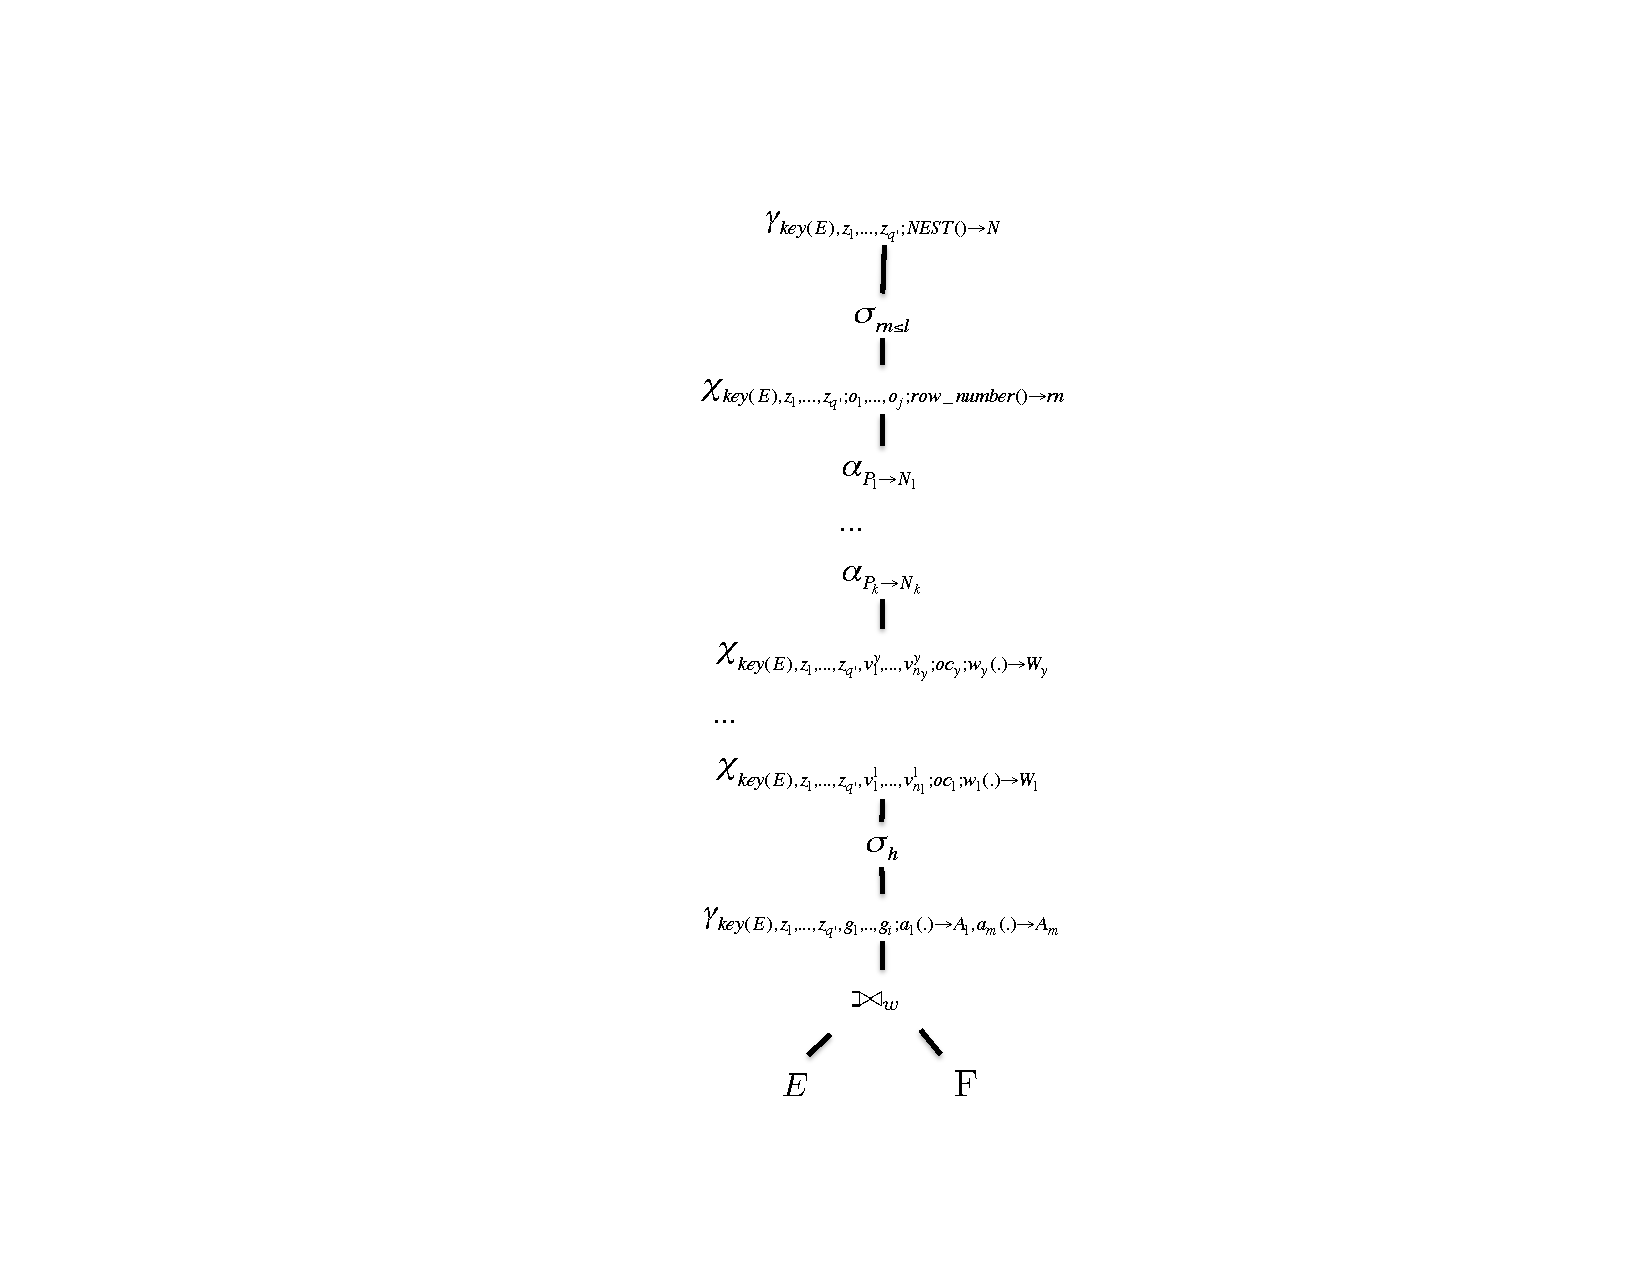
\includegraphics[width=0.65 \linewidth]{images/R4.pdf}
\end{figure}


% \section{Scenarios}

% In this section, we consider subclasses of queries from our section 3 rewriting. We show in proof 
\jules{The above claim has not been confirmed yet, as all proofs are not yet provided}.

For each subclass, we make assumption on the cardinalities of the result of the expressions $E$ and $F$. We also make assumptions on the number of distinct values $V(C,E)$ and $V(C,F)$. Note here that by value in this context we mean the set of values taken by every correlated attribute for a given tuple (i.e. $C^t = \{c_1^t, \dots, c_n^t\}$ for some given tuple $t$). 

Each scenario considers a subset of the rewriting pattern seen in section 3.

\subsubsection{Scenario 1}

This scenario corresponds to cases where the query has a potentially small output 

\begin{align}
& \alpha_{P(e.c_1, \dots, e.c_n) \rightarrow N}(E_e) \\
P : & \pi_{p_1,\dots,p_q}(\sigma_{e.c_1 = f.c_1 \vee \dots \vee e.c_n = f.c_n \vee w'}(F_f))& \nonumber
\end{align}

$E < M$

\subsubsection{Scenario 2}

\begin{align}
& \alpha_{P(e.c_1, \dots, e.c_n) \rightarrow N}(E_e) \\
P : & \pi_{p_1,\dots,p_q}(\lambda_l\tau_{o_1,\dots,o_l}(\sigma_{e.c_1 = f.c_1 \vee \dots \vee e.c_n = f.c_n}(F_f)))& \nonumber
\end{align}

\subsubsection{Scenario 3}

We consider two scenarios which follows the same algebraic form, but different database instance characteristics. 

\begin{align}
& \alpha_{P(e.c_1, \dots, e.c_n) \rightarrow N}(E_e) \\
P : & \pi_{p_1,\dots,p_q}(\gamma_{g;a(.) \rightarrow A}(\sigma_{e.c_1 = f.c_1 \vee \dots \vee e.c_n = f.c_n}(F_f)))& \nonumber
\end{align}

\subsubsection{Scenario 4}

\begin{align}
& \alpha_{P(e.c_1, \dots, e.c_n) \rightarrow N}(E_e) \\
P : & \pi_{p_1,\dots,p_q}((\lambda_l\tau_{o_1,\dots,o_l}(\gamma_{g;a(.) \rightarrow A}(\sigma_{e.c_1 = f.c_1 \vee \dots \vee e.c_n = f.c_n}(F_f))))& \nonumber
\end{align}

In table \ref{tab:matching}, we describe how those scenarios relate to "real world" use cases.


\begin{table}[]
\centering
\caption{Matching scenarios for each use case}
\label{tab:matching}
\begin{tabular}{|l|l|}
\hline
Use Case               & Matching Scenarios    \\ \hline
Hadoop ETL              & $S3$ \\ \hline
BDAS                    & $S4$ \\ \hline
Analytics Visualization & $S1, S2$ \\ \hline
Web Services \& APIs    & $S1, S2$ \\ \hline
\end{tabular}
\end{table}


\section{Cost Model}

We show that the proposed rewriting leads to better performance in a large variety of "real-world" data analytics scenarios. In this section, we present an abstract analysis of the cost of the TAAT, NSAAT and DSAAT algebraic formulations on execution environments typically utilized for those scenarios. For this purpose, we introduce a theoretical cost model focused on network overhead and disk access  based on a number of (listed) assumptions regarding network, storage, indices and relational operators which are common across those execution environments.

\begin{figure}[h]
\centering
\caption{Query Processor Architecture \label{fig:architecture}}
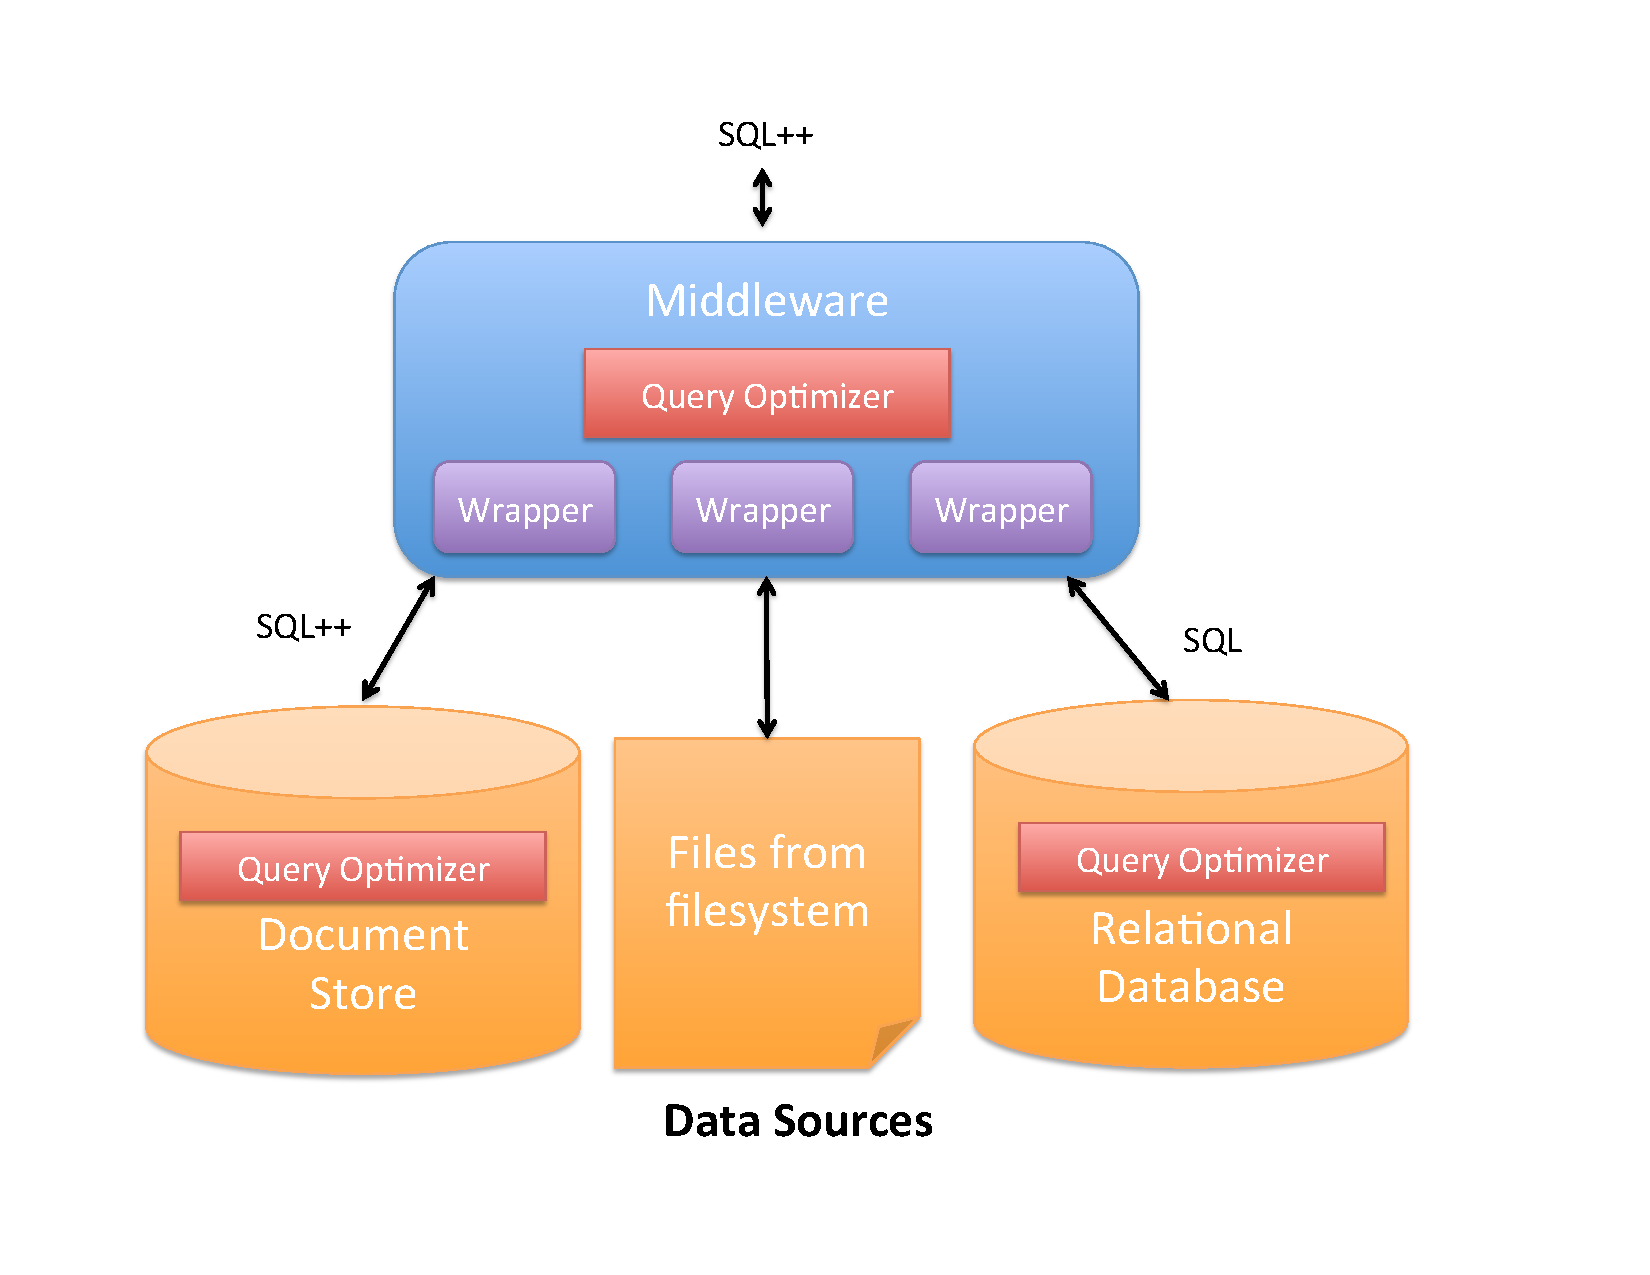
\includegraphics[width=\linewidth]{images/Architecture.pdf}
\end{figure}

\subsection{Setup}

\subsubsection{Execution Environment}

We argue the query rewriting presented in this paper has value on a variety of different query processors for semi-structured data. We consider two broad categories of query processors: document stores and data integration middlewares. We evaluate the performance improvement of our rewriting using a theoretical architecture (shown on figure \ref{fig:architecture}) which is representative of both categories. This architecture has two components: a data processing \emph{middleware}, and a set of zero or more \emph{data sources} with various levels of \emph{capabilities}.

\textbf{Middleware}: the data processing middleware answers SQL++ queries by executing algebraic plans over the data sources. It is capable of processing any SQL++ algebraic operator. To process SQL++ algebraic operators, the middleware has access to a number of physical operators (algorithms) which are listed on table \ref{table:op-costs}. The middleware also has access to a query optimizer, which allows it to choose which physical implementation to use for processing of a given algebraic operator. It is also capable of delegating a portion or all of the plan to a data source, if : 1) the data source is capable of processing all operators in that plan and 2) all stored collections accessed in that plan are located at that data source. Once a plan is delegated to a datasource, the wrapper for that datasource converts the algebraic plan into a query expressed in that datasource's native query language.

\textbf{Data Sources}: they contain the data queried by the middleware. We consider here only three kinds of data sources: a file system, a traditional relational database system and document stores. Each data source has its own set of characteristics which we describe next:

\begin{itemize}
\item{\textbf{File System}: Any file system which is accessible by the middleware process. This source is not capable of processing any SQL++ operator.}
\item{\textbf{RDBMS}: Any relational database system which has access to the physical operators shown on table \ref{table:op-costs}. For simplicity, we do not assume the RDBMS has access to any other physical operators. An RDBMS is only capable of processing \emph{purely relational} operators. By purely relational, we mean operators whose output are regular rows of atomic scalars (i.e. they do not contain any nesting or heterogeneity).}
\item{\textbf{Document Store}: we consider any document store which is capable of processing any SQL++ algrebraic plan. We assume the document store  also has access to the physical operators shown on table \ref{table:op-costs}. In the case where the document store is the single datasource, we consider the middleware optional (the user may query using the document store directly).}
\end{itemize} 

We assume that all query processors considered to be using single machine setups. We do not consider the cases where operators can run as parallel tasks of a cluster in a share-nothing architecture. We also assume all databases (including the middleware) have the ability to spill to disk in case the size of an intermediate results exceeds the available memory. In practice, document stores as well as integration middlewares employ complex optimizations that cannot be comprehensively accounted for in an analytical model. As such, the computation costs and associated speedups reported in this section should be used as rough estimates of the actual cost.

The middleware answers queries from a single source at a time (i.e. we do not consider complex cases where the data is joined from multiple source in the middleware). This assumption is of particular importance when 

\jules{@Yannis: I see a problem here when we reach experiments. I only know two kinds of middlewares (FORWARD middleware and Informatica), none of which can spill to disk without invoking a "supporting" database.}

\subsubsection{Notations}

\begin{itemize}
\item A plan context $P[]$ denotes a plan with one "hole"; i.e. a plan in which an $n$-ary operator has $n-1$ operators and a special character $[]$ as children, and $P[Q]$ represents the plan $P$ in which the hole has been replaced with the subplan $Q$. For example, for $P[] = \pi_p([])$ and $Q = \sigma_w(R)$, we have $P[Q] = \pi_p(\sigma_w(R))$.
\item $cost(P)$ denotes the cost of executing a plan $P$ and $cost(P[],Q)$ denotes the cost of executing the plan $P[Q]$ assuming $Q$ has already been evaluated and its result is accessible is accessible at no cost.
\item $network(P)$ denotes the cost of sending the result of $P$ to a target database system through a network with throughput $K_n$. Notice that we only consider "internal" network cost. For example, in the Hadoop ETL setting, we do not consider the cost of sending the end result to the target database. 
\item $|P|$ denotes the number (resp. average number) of binding tuples outputted by a subplan (resp. correlated subplan) $P$. Conversely $\#_f(P)$ is the number (resp. average number) of memory frames required to store the result of subplan (resp. correlated subplan) $P$. Thus we have $\#_f (E) = \ceil{\frac{|E|.T_E}{f_s}}$, where $T_E$ is the tuple width and $f_s$ is the frame size. In the remaining of the paper, we approximate this expression to $\#_f(E) = \frac{|E|}{f_s}$. \jules{This approximation could cause a problem, since tuples containing nested collections may have arbitrary size and ignoring this can lead to incorrect size estimates. Likewise, one of the advantages of NSAAT over DSAAT is the decrease in tuple width, which this assumption would eliminate.}
\item $attr(E)$ denotes the set of attributes in the output of expression $E$.
\item $join\_size(E,F,w)$ denotes the size of the output (in memory frames) of a join with condition $w$. We have $(E,F,e.c = f.c \cap w')) = \#_f \frac{|E| |F|}{max(V(c,E),V(c,F))} s_{w'}$, where $c \in attr(E) \cap attr(F)$ and $s_{w'}$ is the selectivity of the condition $w'$. Notice that we do not distinguish between the size of the output of an inner and the outer join.
% \item Denote $R_g$ the group of tuples in the output of $R$ with grouping attribute values equal to $g$ for some $g$.
\item Aggregation functions are said to be $bounded-state$ if the size of their output is bounded. Traditional aggregation functions such as \texttt{COUNT(.)} and \texttt{AVERAGE(.)} belong to this category, while \texttt{NEST(.)} does not, since the size of its output grows with the size of its input.
\item We denote $M_{DB}$ as the memory budget for each operator in database system $DB$ (e.g. $M_{PostgreSQL}$ when considering the PostgreSQL system). This memory budget is expressed in terms of number of memory frames. We assume all operators in a given database system are entitled to the same memory budget. In cases where there is only one database system for an execution environment, we simply say $M$.
\item We denote $V(c,E)$ as the number of distinct values of attribute $c$ in the output of expression $E$.
\item We call the \emph{reach} of a query the amount of data which \emph{must} be read from database instance in order to accurately answer a query, while in the presence of all possible indices.\jules{I would be surprised if I am the first to ever introduce this term.}
\item We denote $merge(R)$ as the cost of sorting using the merge-sort join technique beyond the first pass.  Note that $merge(R) = \#_f(R)$ when $R < M^2$ (only two passes).
\end{itemize}

\begin{table*}[t]
\centering
\caption{Operator Costs \label{table:op-costs}}
\begin{tabular}{|c|C{2.5cm}|C{3cm}|C{2.5cm}|C{3cm}|}
\hline
Physical Operator / Color Code & Read Cost & Transform Cost & Write Cost  & Restrictions / Characteristics \\ \hline
$ T \leftarrow R$ (Copy) & $\#_f(R)$ & 0 & $\#_f(R)$ &  \\ \hline
$\sigma_w, \pi_p, \lambda_l$ &  0 &  0 & 0  & pipelined  \\ \hline
$ Scan^{\textbf{sequential}}(R)$ & $\#_f(R)$ & 0 & 0 & \\ \hline
$ Scan^{\textbf{index}}_{c_r = X}(R)$ & $\frac{|R|}{V(c,R)}$ & 0 & $\#_f(\frac{|R|}{V(c,R)})$ & $R$ is a table, $c_r \in attr(R)$, index on $R.c$ and $X$ is a scalar  \\ \hline
$Join^{\textbf{memory\_hash}}_{c_r = c_s}(R,S)$ & $ \#_f(S) + \#_f(R)$ & 0 & $join\_size(R,S,w)$ & $\#_f(R) < M_{DB}$, $R$ already loaded in memory  \\ \hline
$Join^{\textbf{right\_index}}_{c_r = c_s}(R,S)$ & $\#_f(R)$ & $|R| \frac{|S|}{V(c,S)}$ & $join\_size(R,S,w)$ & $\#_f(R) < M_{DB}$, $R$ already loaded in memory   \\ \hline
$Join^{\textbf{sort\_merge}}_{c_r = c_s}(R,S)$ & $\#_f(R) + \#_f(S)$ & $\#_f(R) + \#_f(S) + merge(R) + merge(S)$ & $join\_size(R,S,w)$ &   \\ \hline
$Join^{\textbf{sort\_merge}}_{c_r = c_s}(R,S)$ & $merge(R) + merge(S)$ & 0 & $join\_size(R,S,w)$ & inputs $R$ and $S$ are sorted on join attributes  \\ \hline
% $Join^{reduce-side}_{c_r = c_s}(R,S)$ & ? & ? &  $join\_size(R,S,w)$ & ?  & H  \\ \hline
% $Join^{map-side}_{c_r = c_s}(R,S)$ & ? & ? &   $join\_size(R,S,w)$ & ? &  H \\ \hline
$\tau(R), \chi(R), \gamma_{NEST}^{\textbf{SB}}(R)$ & $\#_f(R)$ & $\#_f(R) + merge(R)$ & $\#_f(R)$  &   \\ \hline
$\gamma_{NEST}^{\textbf{PC}}(R)$ & $\#_f(R)$ & 0 &  $\#_f(R)$ & input $R$ is sorted on $g$  \\ \hline
$\gamma_{BS}^{\textbf{PC}}(R), \delta_{PC}(R)$ & $\#_f(R)$ &  0 & $\#_f(\delta(\pi_g(R))$ & input $R$ is sorted on $g$ \\ \hline
$\gamma_{BS}^{\textbf{SB}}(R), \delta_{SB}(R)$ & $\#_f(R)$  & $\#_f(\delta(\pi_g(R)) + merge(R)$ & $\#_f(\delta(\pi_g(R))$ &   \\ \hline
$\alpha_{P \rightarrow N}(R)$ & $\#_f(R)$ & $|R| cost(P)$ & $\#_f(R)$ & Tuple size increased, number of tuples reduced  \\ \hline
\end{tabular}
\end{table*}

\subsubsection{Assumptions}

To make the analysis simpler, we first make the following assumptions (and discuss them later on):

\begin{itemize}
\item We assume the size of a memory frame $\#_f(F)$ equals the size of a disk block.  This way we have $SeqScan(R) = \ceil{\frac{R.T_R}{B}} = \ceil{\frac{R.T_R}{f_s}} = \#_f(R)$.
\item We only look at the number of blocks, not at the time required to fetch those blocks (not distinguishing between random and sequential IO). 
\item We assume all indices are available and will be used by the query optimizer of the database system if it chooses to do so.
\item We assume no skew in correlation attribute values. This way, we assume that the value of attribute $N$ of a apply plan operator $\alpha_{P(c_1,\dots,c_n) \rightarrow N}$ will have the same size, no matter which values correlated attributes $c_1,\dots,c_n$ take.
\item We assume $\alpha_{P(c_1,\dots,c_n) \rightarrow N}$ are applied sequentially, with the fully memory budget available to \emph{each} execution of the plan $P$.
\item In all scenarios, we assume the size of the result of the inner query (of the query pattern, that is) is expected to be small, given that nesting big collections isn't practical and does not represent a real use case.
\item The \texttt{FROM} clause $F$ of the inner plan $P$ is a join of $n$ stored collections. We assume only one of these collections, denoted with $R$, is correlated with the outer plan through a selection $\sigma_{c_e = c_r}(R)$, where $c_e$ and $c_r$ attributes of $E$ and $R$, respectively. We denote $F'$ the plan context such that $F = F'[\sigma_{c_e = c_r}(R)]$. Finally the expression $rf(F,T)$ is such that the join order of $F$ has not changed. That is, $rf(F,T) = F'[T \innerjoin_{c_e = c_r} R]$.
\item We assume the presence of both \texttt{GROUP BY} and \texttt{ORDER BY} clause in the input nested query. \jules{@Yannis: I believe it is not necessary to explicitly describe queries with either only \texttt{GROUP BY} or only \texttt{ORDER BY} in the nested query separately.}
\item We make the assumption that $\frac{|F|}{M f_s} \leqslant f_s$, which is true anytime $|F|$ is smaller than $f_s$ times the memory size. Given $f_s$ typically ranges in the kB to MB range, this assumption holds unless $|F|$ is bigger than one million times the memory size, which we don't consider realistic in practice.
\item We make the assumption that no stored collection or intermediate result ever exceed $M^2$, which reflects realistic use cases.
\item In the case of an index being used by a $Scan^{index}$ or $Join^{right\_index}$ operator, we assume this index is stored entirely in memory, and does not take space in the memory budget allocated for the query.
\end{itemize}

Note that the running example query follows these assumptions.

\subsubsection{Operators considered}

Our cost model provides a taxonomy of physical operators implementations which can be used to form execution plans (those are shown on table \ref{table:op-costs}). Each row on table \ref{table:op-costs} corresponds to a implementation of a algebraic operator. The cost associated with using this operator is split into three sections: read cost, transform cost and write cost. Write cost is only paid if output is too large to fit in memory and is not the final result. Read cost is paid if input is not already in memory. In case of joins, if one of the inputs is already in memory but not both, then only the cost of reading the input not in memory is paid. Transform cost is paid if size of the input is greater than memory. The cost of the execution of a given operator is the sum of all three costs. Finally, the restrictions column indicates under which conditions can a particular implementation be used. Therefore, we define the \emph{cost} of executing an algebraic operator to be the cheapest cost among competing implementations of that operators which meet the restrictions. 

\subsubsection{Cost Breakdowns}

We next describe precisely the cost breakdown of expressions TAAT, NSAAT and DSAAT. 

\eat{
We assume the SQL++ queries being evaluated exhibit the following pattern :
\lstinputlisting[language=SQL]{code/query_pattern.sql}
Note that within the nested query, we assume presence of both \textt{GROUP BY} and \texttt{ORDER BY} clause. 
}

\begin{equation*}
\begin{aligned}
cost(TAAT) = & |E| (cost(Scan(R)) + cost(F'([]), Scan(R)) + \\
                    & + cost(\tau(\gamma_{inner}([])), F)) \\
\end{aligned}
\end{equation*}

The TAAT plan evaluates $|E|$ times the inner plan $P$, which itself is the addition of the following costs: i) the cost of evaluating the \texttt{FROM} clause (which requires scanning collection $\sigma_{e_c = r_c}(R)$ and joining with other collection in plan context $F'$) and ii) the cost of evaluating the inner \texttt{GROUP BY} (denoted $\gamma_{inner}$) and \texttt{ORDER BY} clauses on the output of the \texttt{FROM} clause.

\begin{equation*}
\begin{aligned}
cost(NSAAT) = & cost(E \rightarrow T) + cost(rf(F,T))   \\
                    & + cost(\gamma_{\texttt{NEST}}(\chi(\gamma_{inner}([])), rf(F,T)) \\
                    & + cost(\leftouterjoin([T,]),r(P,T))  \\
\end{aligned}
\end{equation*}

The cost of evaluating the NSAAT plan is the addition of the following costs : i) the cost of the assignment $E \rightarrow T$ ii) the cost of evaluating $rf(F,T)$ iii) the cost of the $\gamma_{inner}$ aggregation, the $\chi$ partition-based ordering and the $\gamma_{\texttt{NEST}}$ nesting aggregation iv) the cost of the final outer join between $T$ and $r(P,T)$. Note that evaluating $rf(F,T)$ requires performing an inner join between the distinct correlated values fetched from $T$ and the expression $F$ resulting in a the following cost : $cost(rf(F,T)) = cost(\delta(T)) + cost(\innerjoin([,R]),\delta(T)) + cost(F'([]), \innerjoin(\dots))$. 

\begin{equation*}
\begin{aligned}
cost(DSAAT) = & cost(F) + cost(\leftouterjoin([E,]),F) \\
                   & + cost(\gamma_{\texttt{NEST}}\chi(\gamma_{inner}([])), \leftouterjoin(
                   \dots)) \\
\end{aligned}
\end{equation*}

Finally, the cost of evaluating the DSAAT plan is the addition of the following costs: i) the cost of expression $F$, ii) the cost of the initial outer join between $E$ and $F$ iii) the cost of the $\gamma_{inner}$ aggregation, the $\chi$ partition-based ordering as well as the $\gamma_{\texttt{NEST}}$ aggregation.

Note that these costs assume that selection pushdown and cross-product removal optimizations have already occurred. Given the cost of computing expression $E$ is paid no matter what, it is not included in the above cost expressions. Note as well that pipelined operators ($\lambda$, $\sigma$ and $\pi$) are not included either. Finally, some systems may introduce additional costs to those expressions, such as network costs in middleware settings.

\subsection{Scenarios}

We next evaluate the performance of the TAAT, NSAAT and DSAAT algebraic formulations in three different scenarios.  For each scenario, we describe the characteristics of the query pattern and then discuss and compare the cost of the expressions for different ranges of $V(c_e,E)$ and $V(c_r,F)$, the number of distinct correlated attribute values for expressions $E$ and $F$, respectively. Finally, we summarize the cheapest implementations for each scenario in the appendix cost tables \ref{table:r0}, \ref{table:r2} and \ref{table:r4}.

\subsubsection{Scenario 1: Large Reach, Small Output}

This situation is typical of analytical intelligence use cases, in which human analysts query large datasets and read the results of their queries to obtain valuable insight. The running example scenario belongs to this category. 

\begin{itemize}
\item{The result of such use cases are typically small (thus the "small output"), since they have to be human-readable. As a result, the size of $E$ is expected to be tiny in database terms (may be less than 100). In this situation, the cost $E \rightarrow T$, $\delta(T)$ and $\gamma_{\texttt{NEST}}$ are insignificant.}
\item {The expression $F$ could be very large (thus the "large reach"), and exceed the memory budget $M$ many times.}
\end{itemize}

\subsubsection{Scenario 2: Large Reach, Large Output}

This situation is typical of ETL use cases, in which large datasets are transformed and loaded into semi-structured databases. 

\begin{itemize}
\item{The aim of such use cases is too transform large quantities of data in a single query. The result of such use cases may be well beyond a human readable size. As a result, the size of $E$ is expected to be very large. In this situation, the cost $E \rightarrow T$, $\delta(T)$ and $\gamma_{\texttt{NEST}}$ become significant.}
\item {The expression $F$ could be very large (thus the "large reach"), and exceed the memory budget $M$ many times.}
\end{itemize}

\begin{figure*}[h]
\centering
\caption{Physical Query Plans \label{fig:plans}}
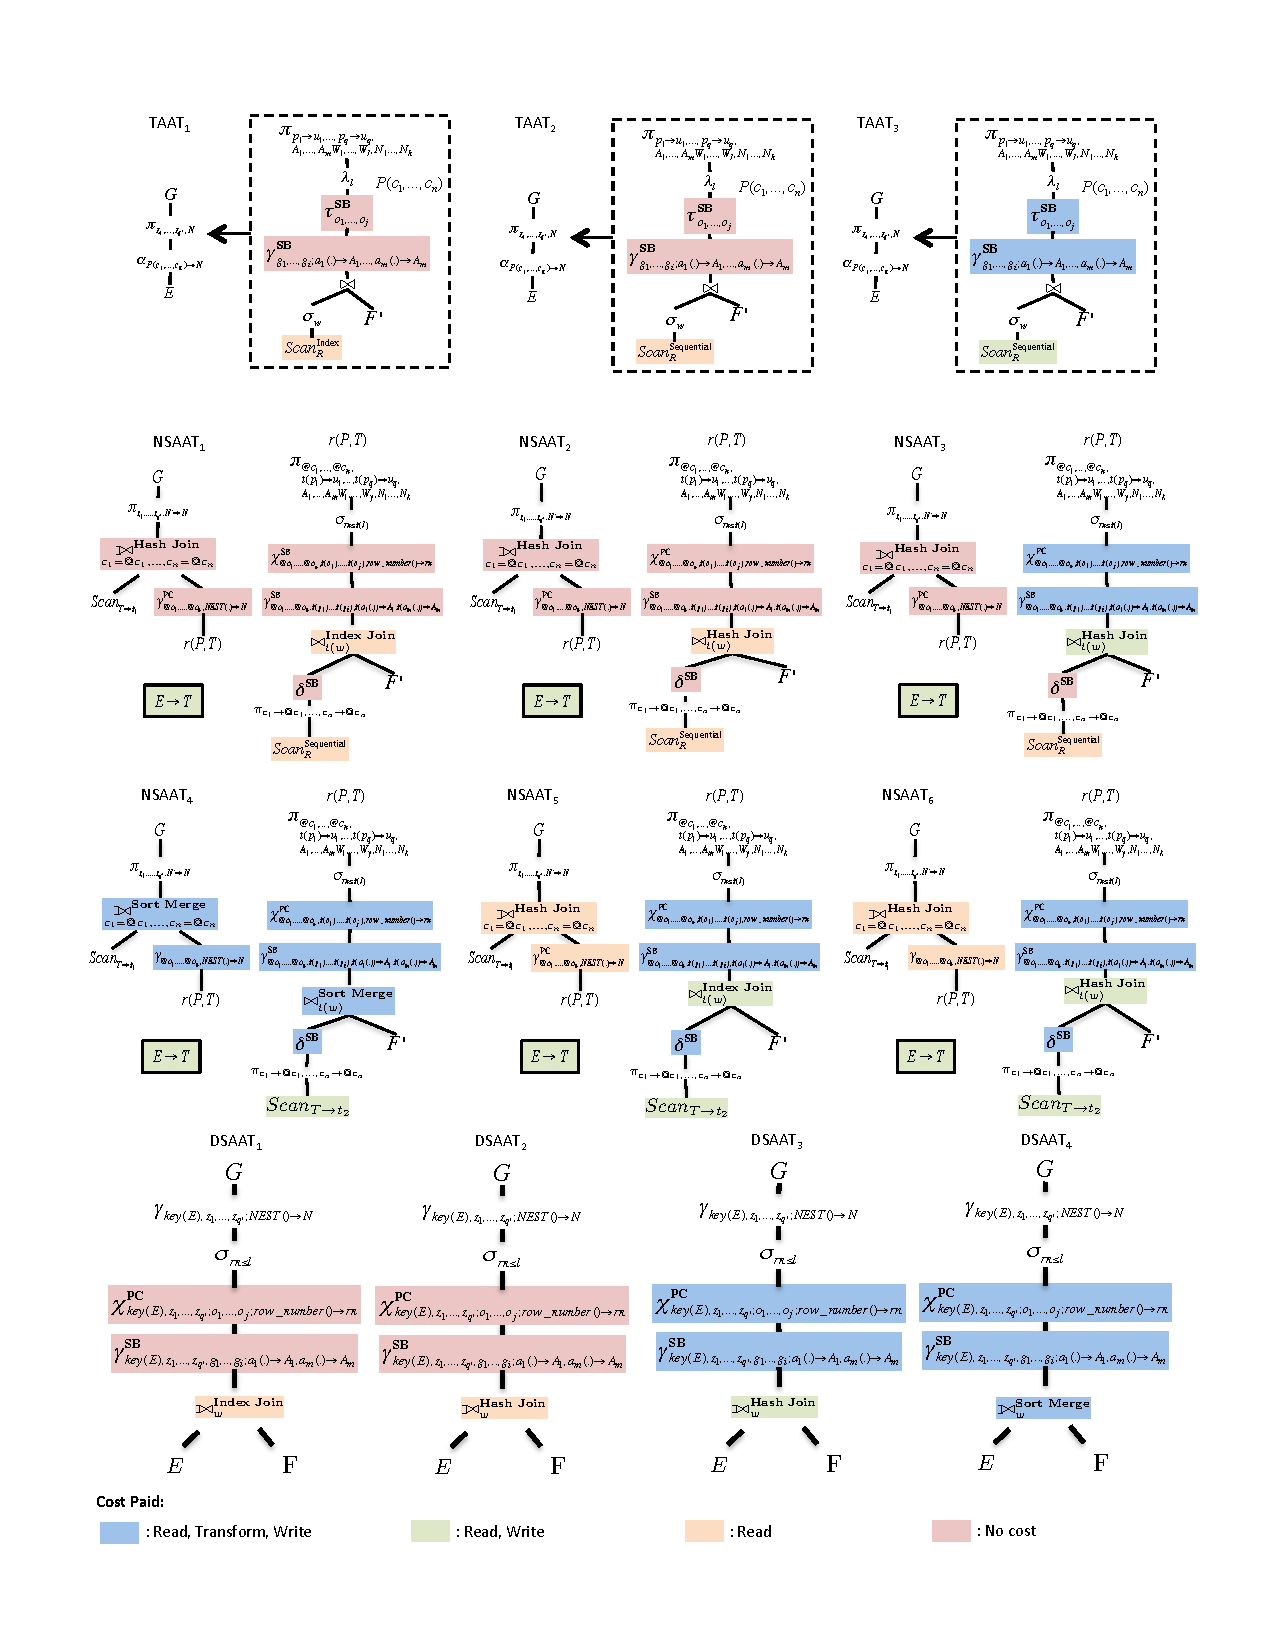
\includegraphics[width=\linewidth]{images/PhysicalPlans.pdf}
\end{figure*}

\subsection{Document Store}

The physical plans produced by the query optimizer for each formulation are shown on figure X.

\subsubsection{Scenario 1}

\subsubsection{Scenario 2}

\subsection{Middleware}

\subsubsection{Scenario 1}

\subsubsection{Scenario 2}

\jules{Index join is only if possible if $n$ is 1}

\eat{
\textbf{Discussion}: on figure \ref{fig:scenario1} of appendix \ref{app:cost}, we display the cost of each formulation for different ranges of $V(c_r,F)$ (number of distinct correlated attribute values), assuming the query optimizer picks the cheapest option for every operator. All values within the same range result in the same physical implementations being chosen as by the query optimizer. We discuss specific ranges further:

% Discuss borders
\begin{itemize}
\item When $f_s \leqslant V(c_r,F)$,  expressions $\sigma_{c_e=c_r}(F)$ and $\innerjoin_{c_e=c_r}(E,F)$ have high selectivity and small output, resulting in the use of index joins/scans and in-memory sorting for all subsequent $\gamma$, $\tau$ and $\chi$ operations. In this situation, TAAT loses big given the cost of $F'$ may be significant, since $F'$ would has to be paid $|E|$ times more than on NSAAT, DSAAT. NSAAT is cheaper than DSAAT, but only marginally, because NSAAT's index join is executed on fewer tuples than DSAAT's. \textbf{Result}: NSAAT < DSAAT < TAAT.
% Otherwise, costs for all expressions are roughly the same, since $V(c,E) \simeq |E|$ when $E$ is small.
\item When $V(c,F) \leqslant \frac{|F|}{M f_s}$: expressions $\sigma_{c_e=c_r}(F)$ and $\innerjoin_{c_e=c_f}(E,F)$ are not selective and have even larger outputs, which results in sequential scans or hash-joins being used, as well as external sorting. In this situation, TAAT is the most expensive, while NSAAT is only marginally cheaper than DSAAT, again due to $V(c,E) \simeq |E|$. \textbf{Result}: NSAAT < DSAAT < TAAT.
\item When $\frac{|F|}{M f_s} \leqslant V(c,F) \leqslant f_s$: the cheapest formulation depends on the parameters found on figure \ref{fig:scenario1}. Of particular interest are the boundaries $\frac{|F|}{M f_s}$, $\frac{V(c_e,E)|F|}{M f_s}$ and $\frac{|E||F|}{M f_s}$, which determine whether a formulation can rely on in-memory sorting or has to resort to an external sort to process the \texttt{GROUP BY} and \texttt{ORDER BY} clauses. In particular, the TAAT formulation can rely on in-memory sorting for lower values of $V(c_r, F)$. This is possible because of the following: while the TAAT formulation has to sort $|E|$ times, each result to be sorted is $|E|$ times smaller than in its set-at-a-time counterparts.
\end{itemize}
}


\section{Experimental Evaluation}

To be filled in later.


\section{Use Cases}

The rewriting we present is useful in a wide variety of uses cases, with very different execution environments and query characteristics. We distinguish at least four use cases: 1) an ETL framework used for operational intelligence 2) A big data analytics system used by business intelligence users, 3) a web application which provides analytics visuals for a browser and 4) a cloud web service/API for external applications.


\subsection{Operational Intelligence}

Operational Intelligence applications collect machine generated data from logging systems and/or application output for the purposes of monitoring and real-time analytics. It involves two distinct tasks: collecting data, then analyzing it. It is often the case that the database systems used for collection and analysis are distinct, and data must be moved from the former to the latter through the use of ETL tools. 
% 

% Describe query characteristics
It is also often the case that the system used for analysis is a document store such as MongoDB \eat{\jules{find sources which describe why document stores are good for this kind of analysis}}, which stores data as documents with nested structures. One example is clickstream analysis for an online website. To facilitate further analysis, an ETL middleware pre-aggregates daily, hourly and minute hit counts for every web page from a source log file into a target document database using query \ref{list:query2} from appendix \ref{app:examples}. 

\eat{
These stores benefit particularly well from our rewriting, since it targets the queries which are used to produce this nesting.
\begin{figure}[h]
\label{fig:hadoop}
\centering
\caption{Hadoop ETL architecture}
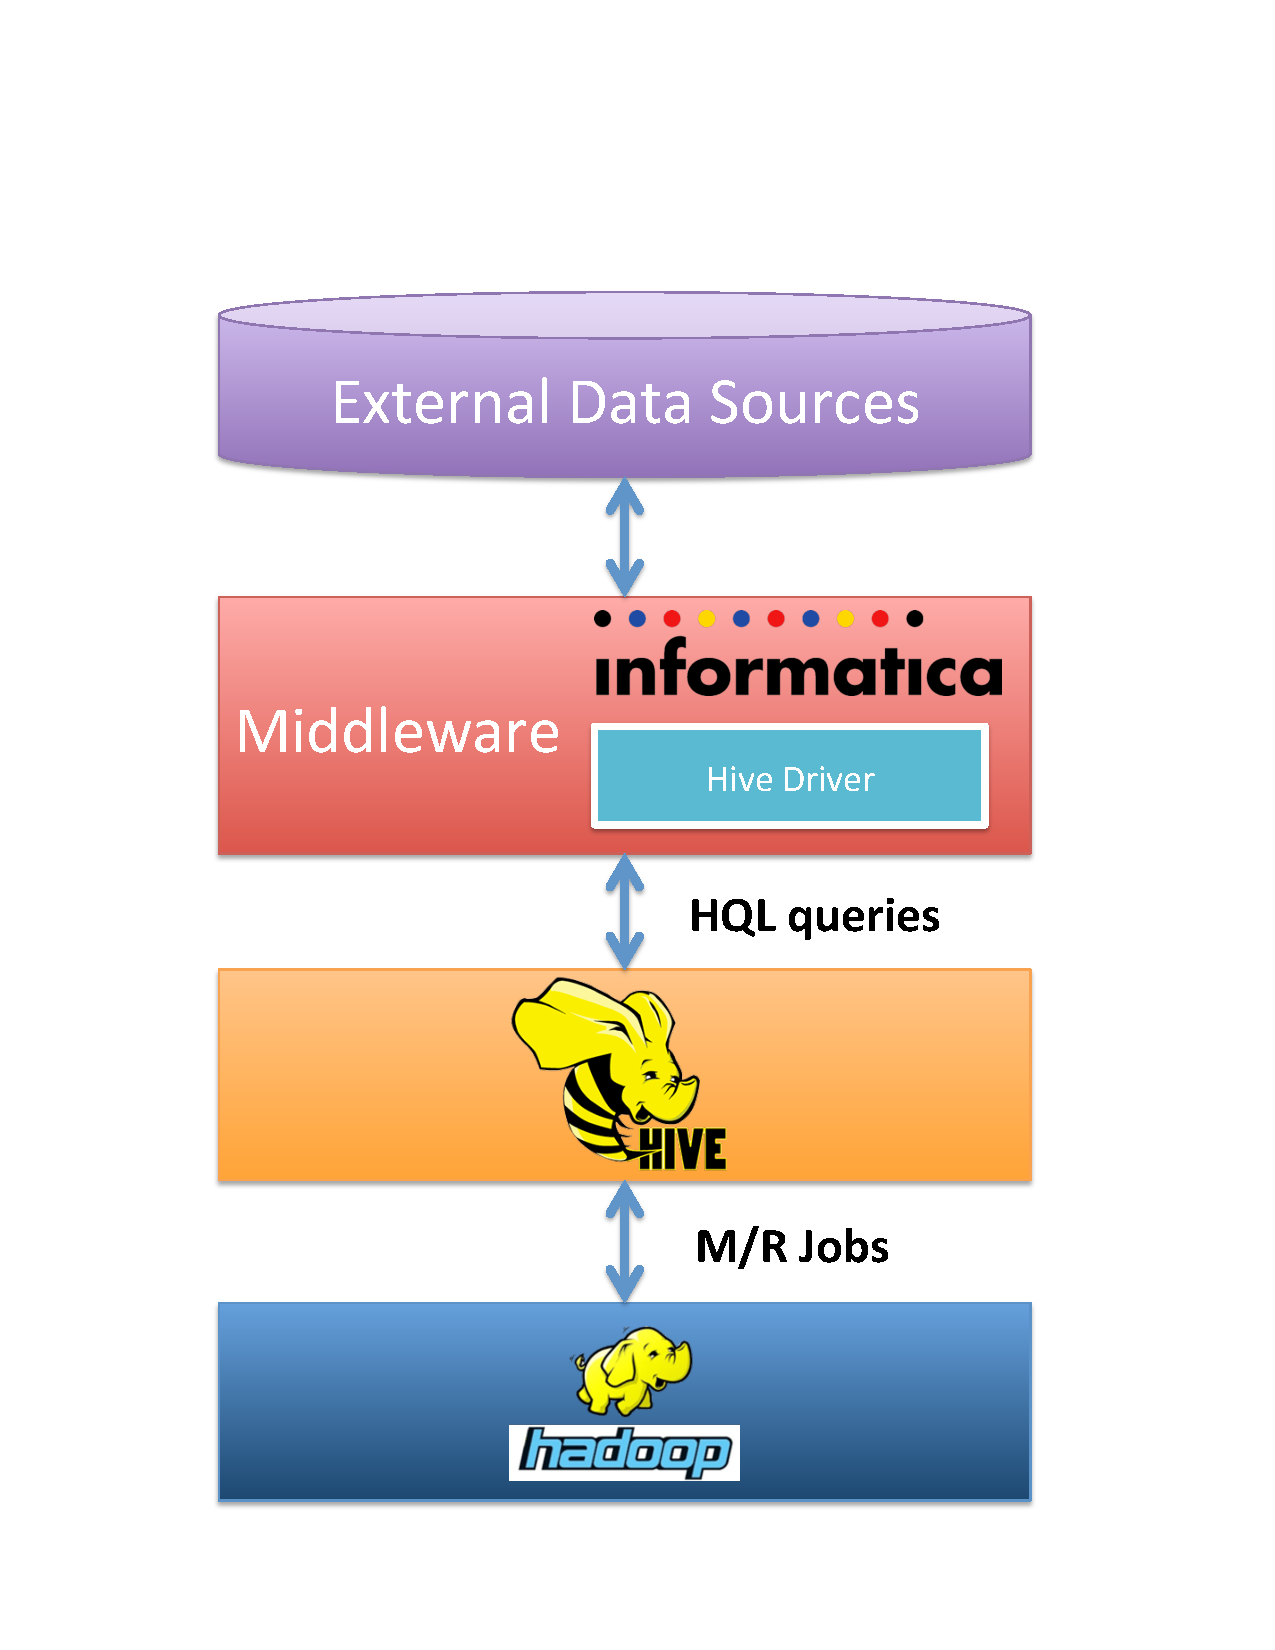
\includegraphics[width=5cm]{images/HadoopETL.pdf}
\end{figure}

% Describe execution environment
On figure \ref{fig:hadoop} is shown the architecture used by Informatica's Big Data Edition product \cite{informaticaBDE}, a commercial ETL middleware with (potentially) access to a Hadoop cluster. In the operational intelligence use case, the ETL tool will move data from a data source (for example a large log file) to a data target such as MongoDB. The middleware possesses its own query processing capabilities, but can delegate a particular processing task to a Hadoop cluster (through Hive) when the data to be processed is too large to fit in the middleware's memory.
}

\subsection{Big Data Analytics System (BDAS)} 

Business intelligence analysts need to make queries for historical and analytical intelligence.  Business intelligence query results are meant to be readable, therefore are small  (a few hundred of rows at most) and typically look at the top-k elements which match a particular criteria. Very fast latencies are not typically a requirement for these kinds of queries, but they sift through very large amounts of data. The number of such queries issued is also expected to be small, given that the number of analysts studying the same dataset at the same time is typically limited.

The execution environment utilized in this use case have typically been parallel data warehouses. However, such systems are inadequate when the result of the formulated queries contain nested collections. For example, consider the following query performed on top of a large retail store dataset: Find the top 30 products that are mostly viewed together with a given an input list of products in an online store \footnote{corresponds to the query 2 from the TPCx-BB benchmark} (query \ref{list:query3} from appendix \ref{app:examples}). For each product in the input list, a collection of 30 products must be found. A new breed of system used when this happens in such cases semi-structured (and parallel) databases, such as AsterixDB.

\eat{
\begin{itemize}
\item Systems built on top of Hadoop (such as Hive) are being used in such cases.
\item Semi-structured parallel query execution engines, such as AsterixDB.
\jules{list might be incomplete}
\end{itemize}

\jules{Should discuss AsterixDB architecture here.}
We argue our rewriting is useful for such BDAS systems with a semi-structured data model. For example, take query \ref{list:query3} from appendix \ref{app:examples}. This query is a typical example of analytical intelligence written by business analysts on a large retail store dataset. Notice that example \ref{list:query3} is exactly an instance of the scenario 4 pattern studied in section 5. 
}

\subsection{Analytics Visualization}

This use case applies to queries issued by analytics/reporting web applications which display nested, aggregated data. Query results for this use case are small enough to be displayed on a computer screen. Moreover, applications tend to have short latency requirements (less than a second) and a large number of users, each requesting multiple distinct visualization renderings as they interact with various UI widgets. As such, visualization queries tend to be numerous and are usually based on small datasets or pre-aggregated data.

For example, consider an analytics web application for a large retail company, which provides its regional and store managers with visuals to help them assess the performance of the clerks working in their store. The application has checkboxes to select clerks working in store $X$, and produces details about the top $K$ largest orders, in terms of total sales price (query \ref{list:query4} from appendix \ref{app:examples}). For each clerk in the selected list, a collection of $K$ orders must be retrieved.

\subsection{Online Web Services \& APIs}

This use cases applies to online web services, typically hosted in the cloud, which provides information to be consumed by external services, such as mobile applications or other web services. Three commercial examples of such services would include:

\begin{itemize}
\item Algolia: a full text search web service, which stores and indexes customer text data (such as product reviews), and provides an API to query it.
\item Keen.IO: a web service which embeds a visual analytics client on the customer's website, and collects/stores the customer data to be visualized.
\item Loggly: a log management web service, which stores and indexes customer logs and allows customers to easily query and visualize them.
\end{itemize}

These web services share a number of characteristics: their queries have typically a low latency requirements, the number of queries answered is large (given each customer can issue an arbitrary number of queries), their APIs only allow a narrow set of highly specialized query patterns and their query results are structured with nesting for program consumption (typically using the JSON data format). Consider a case in which the Loggly web service is used by some large retail website customer. In order to help the customer sift through its page view log, Loggly would provide the per-minute and per-hour page view hit-counts for any given page upon request (query \ref{list:query1} from appendix \ref{app:examples}). The result would produce one tuple per hour, while each minute hit count would be stored in a nested collection field in the corresponding hour tuple. 



\section{Related Work}

To be filled in later.


\bibliographystyle{abbrv}
{
%\scriptsize
\bibliography{main}
}

\appendix

\begin{appendices}
  \section{Cost Tables} \label{app:cost}
  \jules{In table \ref{table:r0} and \ref{table:r2}, external sorts also include spilling and reading back from disk in between the two sorts.}
  
\begin{table*}[]
\centering
\caption{TAAT plan cost table}
\label{table:r0}
\begin{tabular}{|c|c|c|c|}
\hline
Costs & Scenario 1 & Scenario 2 & Scenario 3 \\ \hline

0A: $\sigma(R)$  &  
 $\begin{aligned} & |E| Scan^{index} & \text{if } f_s \leqslant V(c_r,F) \\ & |E| Scan^{Sequential} & \text{else}\end{aligned}$ & & \\ \hline

0B: $F'[], \sigma(R)$ &  $|E| (n-1 \text{ joins})$      &            &            \\ \hline

0C: $\tau(\gamma_{inner}([])), F$    & 
$\begin{aligned} & 0 & \text{if }  \frac{|F|}{V(c_r,F)} \leqslant M f_s \\ & |E|(2 \text{ external sorts}) & \text{else}\end{aligned}$   & 
&
\\ \hline
\end{tabular}
\end{table*}

\begin{table*}[]
\centering
\caption{NSAAT plan cost table}
\label{table:r2}
\begin{tabular}{|c|c|c|c|}
\hline
Costs & Scenario 1 & Scenario 2 & Scenario 3 \\ \hline

2A: $E \rightarrow T$      &    \text{insignificant}        &            &            \\ \hline

2B: $\delta(\pi_{c_e}(T))$      &     \text{insignificant}       &            &            \\ \hline
      
2C: $\innerjoin([,R]), \delta(\pi_{c_e}(T))$ & 
$\begin{aligned} & Join^{right\_index}_{c_e = c_r}(\delta(\pi_{c_e}(T)),R) & \text{if } f_s \leqslant V(c_r,F) \\ & Join^{memory\_hash}_{c_e = c_r}(\delta(\pi_{c_e}(T)),R) & \text{else} \end{aligned}$ &
      &              \\ \hline

2D: $F'([]), \innerjoin(\dots)$ &    n-1 \text{joins}        &            &            \\ \hline

2E: $\chi(\gamma_{inner}([]), rf(F,T)$ & 
$\begin{aligned} & 0 & \text{if }  \frac{V(c_e,E)|F|}{V(c_r,F)} \leqslant M f_s \\ & 2 \text{ external sorts} & \text{else}\end{aligned}$ &            &            \\ \hline

2F: $\gamma_{\texttt{NEST}}([]), \chi(\dots)$      &  \text{insignificant}       &            &            \\ \hline

2G: $\leftouterjoin([T,])$      &     \text{insignificant}       &            &            \\ \hline
\end{tabular}
\end{table*}


\begin{table*}[]
\centering
\caption{DSAAT plan cost table}
\label{table:r4}
\begin{tabular}{|c|c|c|c|}
\hline
Costs & Scenario 1 & Scenario 2 & Scenario 3 \\ \hline
  4A: $F$    &     $n-1$ joins       &            &            \\ \hline
  
  4B: $\leftouterjoin([E,]),F$    &
  $\begin{aligned} & Join^{right\_index}_{c_e = c_r}(E,F) & \text{if } f_s \leqslant V(c_r,F)  \\ & & \text{ and $F$ is a relation} \\ & Join^{memory\_hash}_{c_e = c_r}(E,F) & \text{else} \end{aligned}$
   &            &            \\ \hline
 4C:  $\chi(\gamma_{inner}([]), \leftouterjoin(\dots) $    &  
  $\begin{aligned} & 0 & \text{if }  \frac{|E||F|}{V(c_r,F)} \leqslant M f_s \\ & 2 \text{ external sorts} & \text{else}\end{aligned}$   &            &           \\ \hline
  4D: $\gamma_{\texttt{NEST}}([]), \chi(\dots)$      &      \text{insignificant}    &            &            \\ \hline
\end{tabular}
\end{table*}

\eat{
\begin{table*}
\centering
\caption{Scenario 1 Total Costs using AsterixDB architecture}
\label{table:scenario1}
\begin{tabular}{|c|C{4.5cm}|C{4.5cm}|C{4.5cm}|}
\hline
 & $V(c,F) \geqslant f_s$ & $f_s \geqslant V(c_r,F) \geqslant  \frac{|F|}{M f_s}$ & $ \frac{|F|}{M f_s} \geqslant V(c,F)$ \\ \hline

$cost(R_0)$ 
& $|E| (\frac{|F|}{V(c,F)} + cost(F')) $
& ? % $|E|(\frac{|F|}{V(c,F)} + 2 \frac{|F|}{V(c,F)f_s} + 5 \frac{V(g,F)}{f_s})$
& $|E| (\frac{ F}{f_s} + 2 \frac{|F|}{V(c,F)f_s} + 5 \frac{V(g,F)}{f_s} + cost(F'))$ \\ \hline

$cost(R_2)$
& $ \frac{V(c,E)|F|}{V(c,F)} + cost(F') $
& ? % $\frac{|F|V(c,E)}{V(c,F)}+ \frac{|F|V(c,E)}{V(c,F)f_s} + 2\frac{|F|V(c,E)}{V(c,F)f_s} + 5\frac{V(g,F)V(c,E)}{f_s}$
& $\frac{F}{f_s} + \frac{V(c,E)|F|}{V(c,F)} + 2\frac{|F|V(c,E)}{V(c,F)f_s} + 5 \frac{V(g,F)V(c,E)}{f_s} + cost(F') $  \\ \hline 

$cost(R_4)$ & $\frac{|E||F|}{V(c,F)} + cost(F)$ 
& ? % $\frac{|E||F|}{V(c,F)} + \frac{|E||F|}{V(c,F)f_s} + 2 \frac{|E||F|}{V(c,F)f_s}  + 5 \frac{|E|V(g,F)}{f_s}$
& $\frac{F}{f_s} + \frac{|E||F|}{V(c,F)f_s} + 2 \frac{|E||F|}{f_s V(c,F)} + 5 \frac{|E|.V(g,F)}{f_s} + cost(F)$ \\ \hline

Winner
& $cost(R_2) < cost(R_4) < cost(R_0)$
& ?
& $cost(R_2) < cost(R_4) < cost(R_0)$ \\ \hline
\end{tabular}
\end{table*}
}

\begin{figure*}
\centering
\caption{Scenario 1 \label{fig:scenario1}}
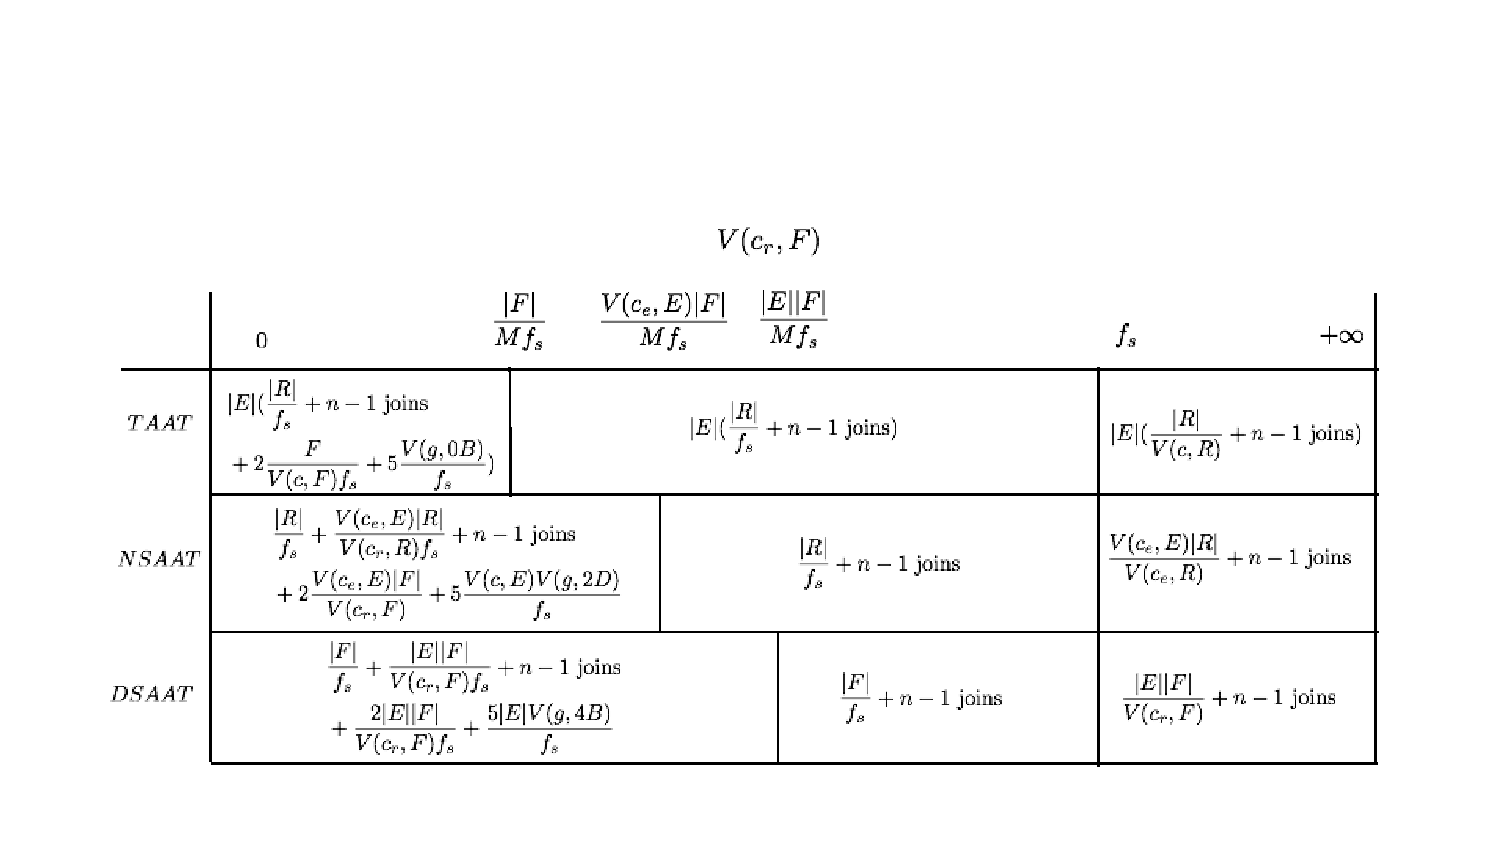
\includegraphics[width=15cm]{images/Scenario1.pdf}
\end{figure*}
  
  
\section{Examples} \label{app:examples}
Here are provided the queries for the use cases given in section 2. Note that all queries are expressed using the SQL++ language developed at UCSD \cite{ong:2014aa}, although those queries would be typically written using an application-specific query language. 

\begin{figure}[h]
\label{fig:schema}
\centering
\caption{TPCx-BB Schema}
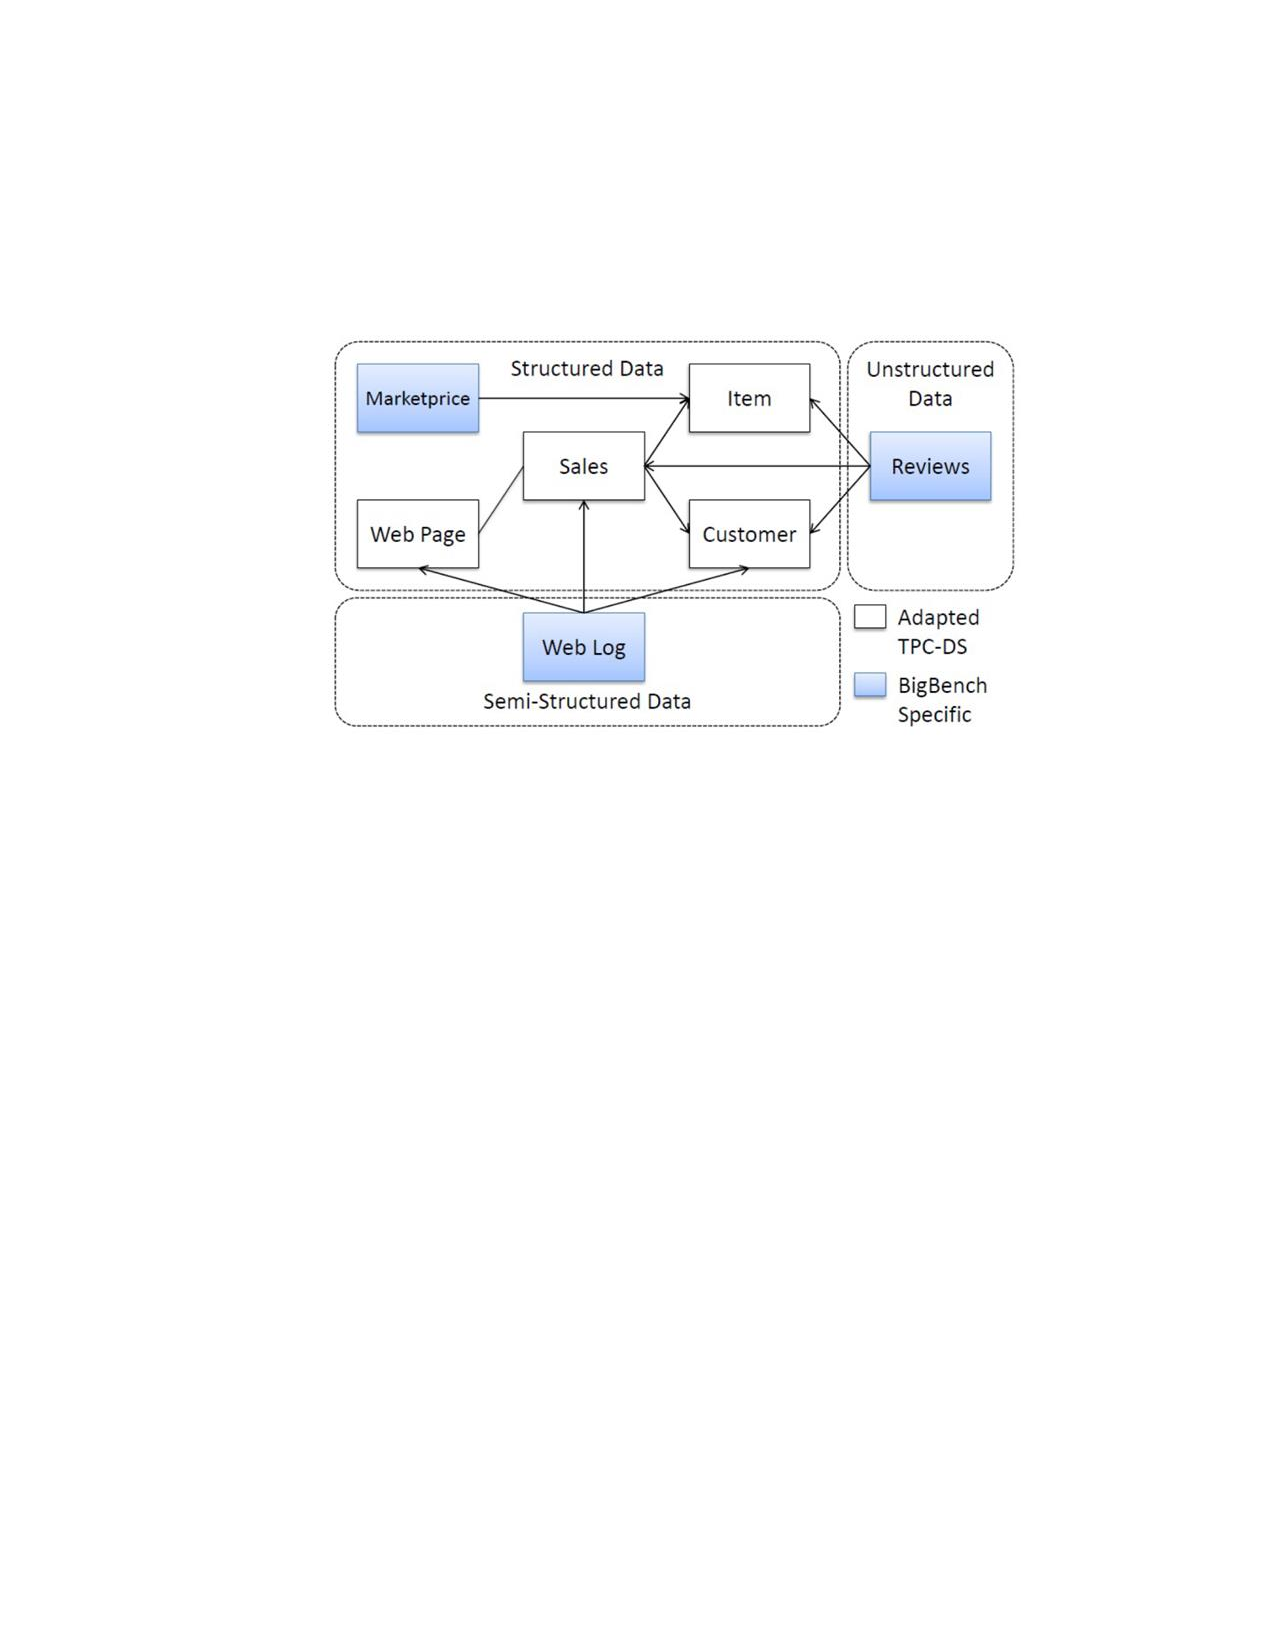
\includegraphics[width=\linewidth]{images/schema.pdf}
\end{figure}

Example \ref{list:query1} produces pre-aggregated hit-counts per minute and per hour for a webpage $Y$ on a day $X$. Example \ref{list:query2} produces this output for all distinct \{day,webpage\} pairs. Examples \ref{list:query1} and \ref{list:query2} are representative of scenarios $S3_S$ and $S3_L$, respectively.
\lstinputlisting[language=SQL,label={list:query1},caption={Operational Intelligence example, local}]{code/query1.sql}
\lstinputlisting[language=SQL,label={list:query2},caption={Operational Intelligence example, global}]{code/query2.sql}

Example \ref{list:query3} corresponds to the query 2 from the TPCx-BB benchmark. It finds the top 30 products that are mostly viewed together with a given list of products in an online store. Note that the order of products viewed does not matter, and "viewed together" relates to a web\_clickstreams \texttt{click\_session} of a known user with a session timeout of 60min.

\lstinputlisting[language=SQL,label={list:query3},caption={TPCx-BB Query 2}]{code/query3.sql}

Example \ref{list:query4} finds, for each clerk from a (small) set of selected clerks working in store $X$, the total price of the top $K$ orders made by that clerk.

\lstinputlisting[language=SQL,label={list:query4},caption={Top orders from the same clerk for selected orders}]{code/query4.sql}

\end{appendices}

\end{document}